% !TEX encoding = UTF-8 Unicode

\linespread{1.7}
\chapter{Modeling of Empirical Transfer Functions with 3D Velocity Structure}
\linespread{2.0}
%\newrefsection
\label{chap:etf}

Empirical transfer functions (ETFs) between seismic records observed at the surface and depth represent a
powerful tool to estimate site effects for earthquake hazard analysis. However, conventional modeling of
site amplification, with assumptions of horizontally polarized shear waves propagating vertically through
1D layered homogeneous media, often poorly predicts the ETFs, particularly, in which large lateral variations
of velocity are present. Here, we test whether more accurate site effects can be obtained from theoretical
transfer functions (TTFs) extracted from physics-based simulations that naturally incorporate the complex
material properties. We select two well-documented downhole sites (the KiK-net site TKCH05 in Japan and
the Garner Valley site, Garner Valley Downhole Array, in southern California) for our study. The 3D subsurface
geometry at the two sites is estimated by means of the surface topography near the sites and information
from the shear-wave profiles obtained from borehole logs. By comparing the TTFs to ETFs at the selected sites,
we show how simulations using the calibrated 3D models can significantly improve site amplification estimates
as compared to 1D model predictions. The primary reason for this improvement in 3D models is redirection of
scattering from vertically propagating to more realistic obliquely propagating waves, which alleviates
artificial amplification at nodes in the vertical-incidence response of corresponding 1D approximations,
resulting in improvement of site effect estimation. The results demonstrate the importance of reliable
calibration of subsurface structure and material properties in site response studies.

%%%%%%%%%%%%%%%%%%%%%%%%%%
\section{Introduction} \label{etf:intro}
Details of how ground shaking is affected by near-surface soil properties can help reduce the uncertainty in stochastic or empirical ground-motion models, which are important components of seismic hazard calculations. Transfer functions (TFs) are widely used to quantitatively represent site response by computing the spectral ratio of ground motions between site and reference locations in the frequency domain \citeg{shearerSurfaceNearsurfaceEffects1987,steidlVariationSiteResponse1993,fieldComparisonTestVarious1995,steidlWhatReferenceSite1996,bonillaBoreholeResponseStudies2002}. Assuming that the reference site, while sharing, approximately, the same path and source with the site of interest, is largely unaffected by site effects,the spectral ratio provided by the TF isolates the site response \citep{borcherdtEffectsLocalGeology1970}. Two types of reference sites, both typically rock, have been proposed: a surface site or a downhole recording (used with the corresponding surface site). The surfacedownhole record pair is valuable for ensuring close proximity of the reference motions at the downhole sensor, ideally located in bedrock, whereas, it may be difficult to find an appropriate reference outcrop site within close distance to the soil site. In this article, we will only analyze TFs computed using surface-downhole site pairs.

The accuracy of site response estimates depends on the accuracy of the subsurface model used, and this is usually assumed to be controlled by the uncertainty in the site properties, in particular, the shear-wave velocity, $V_S$ \citeg{baraniInfluenceSoilModeling2013,griffithsMappingDispersionMisfit2016}. $V_s$ is the most important parameter for conventional 1D modeling of the TF, in which it is assumed that surface (and subsurface) motion consists of horizontally polarized plane S waves propagating through a stack of homogeneous layers \citeg{kramerGeotechnicalEarthquakeEngineering1996}. This modeling procedure (SH1D) ignores the lateral complexity of the often heterogeneous geology and subsurface structure and is, therefore, not able to include potential 2D and 3D amplification effects in the observations \citeg{rotenComparisonObservedSimulated2008,thompsonTaxonomySiteResponse2012}. \citet{zhuSeismicAggravationShallow2018} performed numerical analysis on 2D basins and found that a constant spectral aggravation factor \citep{chavez-garciaComplexSiteEffects2000}, which quantifies the discrepancy between 1D and 2D/3D models, is insufficient to identify basin effects, especially, in close-to-edge regions of shallow basins. Both observations and analytical solutions suggest that 1D models lack an estimate of spatial variability, caused by complex wave propagation such as basin amplification, surface-wave generation, and scattering, and are, therefore, unable to capture spatial correlations, which may be important for understanding risk, especially, to regional-scale infrastructure \citeg{olsenCausesLowfrequencyGround1995,booreCanSiteResponse2004}. Although, recent approaches have attempted to reduce velocity uncertainties in site effect estimation \citep{matavosicPracticesProceduresSitespecific2012,teagueMeasuredVsPredicted2018}, these methods either require prohibitively complex processing or are developed for specific cases only.

It is impractical to constrain subsurface structure over a wide region to the resolution (on the order of meters to tens of meters) required for accurate ground-motion estimation to high frequencies (e.g., 10 Hz). Instead, some studies choose to use simple proxies, based on broad site classes to supplement estimates of soil properties and site spatial characteristics, for example, the National Earthquake Hazards Reduction Program (NEHRP) soil classification \citep{bssc2003NEHRPRecommended2003,akkarEmpiricalEquationsPrediction2010} or a weighted average of $V_S$ in the uppermost 30 m {\citep[$V_{S30}$, e.g., ][]{abrahamsonSummaryAbrahamsonSilva2008,idrissNGAWest2EmpiricalModel2014}. \citet{thompsonTaxonomySiteResponse2012} proposed a scheme to classify surface-downhole site pairs by the extent of interevent variability and goodness of fit between 1D modelling and empirical site response, which can be used to calibrate the constitutive models and guide specific site studies. Despite the use of these characterizations in some generic seismic hazard estimates, for instance, via ground-motion prediction equations, recent work has pointed out the importance of considering site-to-site amplification variability \citep{atkinsonEarthquakeGroundmotionPrediction2006,atikVariabilityGroundmotionPrediction2010}. These studies show that, even within a single NEHRP or $V_{S30}$ class, the variability of site amplification and spatial correlations is strong enough to contribute significant uncertainty in ground-motion estimates.

In this chapter, we propose a method to constrain the near-surface properties using surface topography and perform highresolution 3D numerical simulations to investigate the uncertainty in site response modeling. The simulations naturally take advantage of 3D geotechnical information and are able to incorporate complicated spatially varying amplification effects. We use two downhole array sites, namely the Garner Valley Downhole Array (GVDA) in California and the TKCH05 site from the Kiban–Kyoshin network (KiK-net) surface-downhole pairs in Japan, where detailed in situ constraints of site seismic properties (e.g., $V_S$ and layer thicknesses) and abundant earthquake records are available, for our analysis. Both borehole sites have well-documented geological structure data, and previous studies have showed that SH1D modeling poorly predicts the ground motions without adjustments of subsurface properties or recalibration of constitutive models. \citet{thompsonTaxonomySiteResponse2012} found low interevent variability and poor fit using SH1D modeling for the site TKCH05, due to omission of spatial variability around the site that scatters the downgoing waves and reduces pseudoresonance. They found that no satisfactory fit could be achieved by adjusting the velocity profile, whereas \citet{taoTaxonomyEvaluatingSitespecific2020} showed that modification in the top 20 m can significantly improve the site response estimate for the outcrop TF (spectral ratio between two surface sites). \citet{bonillaBoreholeResponseStudies2002} studied the wave propagation at GVDA and reported significant S-to-P conversions that led to misfit in prediction of the empirical TF (ETF; see \Cref{etf:tfs}) by horizontal-to-vertical spectral ratios. \citet{teagueMeasuredVsPredicted2018} applied the Toro randomization model \citep{toroProbabilisticModelsSite1995} with the spectral analysis of surface waves method, to obtain the site signature with the best match of the ETF and the theoretical TF (TTF); however, this approach suffers from the nonunique nature of inverting $V_S$ profiles.


%%%%%%%%%%%%%%%%%%%%%%%%%%%%%%%
\section{Data}\label{etf:data}

Dependent on the strength of the input motion, site amplification and deamplification can be caused by a combination of linear and nonlinear effects. Here, we focus on linear site effects, and reserve the nonlinear analysis for subsequent research endeavors. To limit our analysis to linear ground motions, we exclude records with maximum surface accelerations larger than 0.1g \citeg{beresnevNonlinearSoilResponse1996}. For each of the two site selections, we randomly picked 36 events of various azimuth and distance to the site that meets this criterion, with a minimum signal-to-noise ratio of five in their records. The goodness of fit between TTFs and ETFs from recordings is described by the variance reduction (VR) as follows:
\begin{equation}\label{eq:etf-1}
  \mathrm{VR}=1-\frac{\sum_{i=1}^{n}\left[\operatorname{TTF}\left(f_{i}\right)-\mathrm{ETF}_{\mathrm{med}}\left(f_{i}\right)\right]^{2}}{\sum_{i=1}^{n}\left[\mathrm{ETF}_{\mathrm{med}}\left(f_{i}\right)\right]^{2}}
\end{equation}
\noindent in which $n$ is the number of frequencies at which the ETFs and TTFs are computed, and ETF med is the median of the ETFs from the events that we selected. We evaluate a set of linearly spaced frequencies between 0.5 and 10 Hz, with the lower limit determined by the noise level of the data, and the upper limit from the resolution of our simulations. The VR ranges within $[-\inf, 1]$, in which VR = 1 means a perfect match, and smaller values indicate poorer fit.

%%%%%%%%%%%%%%%%%%%%%%%%%%%%%%

\section{TFs}\label{etf:tfs}
We compute TFs between surface and downhole locations as follows:
\begin{equation}\label{eq:etf-2}
  TF = \frac{G_s(f)}{G_d(f)}
\end{equation}
\noindent in which $G_s(f)$ and $G_d(f)$ are the root mean squares of the Fourier amplitude spectra of horizontal accelerations at the surface and downhole locations, respectively. It is worthwhile to note that the downhole recordings include the upgoing incident wavefield as well as downgoing waves that are reflected back from the free surface. This phenomenon complicates the wavefields recorded at downhole sites, and, therefore, the use of surface-downhole pairs to study site response. For records obtained at depths shallower than 200 m, as in this study, the upgoing and downgoing pulses overlap in the records, with differences in arrival times as small as 0.2 s, complicating a separation of the two contributions in the presence of extended source duration and site response \citep{shearerSurfaceNearsurfaceEffects1987}. For example, \citet{bonillaBoreholeResponseStudies2002}  found from simulations at the GVDA site using the f -k method that the downgoing wave effect is predominant above the soil-bedrock interface and strongly degraded below that depth. Because it is almost impossible to eliminate downgoing waves from the records, we include the total wavefields at the surface and downhole sites, when calculating the TFs for both synthetics and records.

Our procedure for processing the recorded time series is similar to that documented in \citet{taoInsightsModelingSmallstrain2019}. First, we collected acceleration time series at the surface and downhole accelerometers. Second, a fifth-order Butterworth filter, with a passband of 0.5–12 Hz, was applied to the demeaned and detrended accelerations, in which signal at frequencies below 0.5 Hz was discarded to minimize the contribution from low-frequency noise interference. Third, a second-order polynomial baseline correction was applied to the observed displacement time series, obtained by integrating the accelerations twice. Then, the ETFs were obtained as the ratio of the Fourier spectral amplitude between the surface and downhole acceleration time series for all the events. We further smoothed the TFs using the Konno–Ohmachi smoothing window in the frequency domain \citep{konnoGroundmotionCharacteristicsEstimated1998}. Although, not necessary for the synthetics, we applied the preprocessing (steps 2 and 3) to both synthetics and data for consistency.


\section{Model Construction}\label{etf:model}
It is reasonable to assume that, in the vicinity of a site of interest, bedrock depth varies in accordance with surface topography. In such models, sites located in a mountainous area have near-zero bedrock depth, whereas, sites in valley regions are characterized by larger depths to bedrock. Under this assumption, our 3D mesh is generated by mapping the topography to bedrock depth, with the constraints from borehole logging measurements. Oftentimes, bedrock depth increases
rapidly from the edge toward the center of a sedimentary valley and approaches a maximum near the center of the valley, suggesting that depth to bedrock in a valley can be estimated using the topographic signature from digital elevation models. \citet{gallantMultiresolutionIndexValley2003} proposed an algorithm that operates at multiple scales and combines topographic elevations into a single continuous multiresolution index of valley bottom flatness (MRVBF). Values of MRVBF below 0.5 represent areas with the steepest topography, values between 0.5 and 1.5 relate to the steep areas with few flat valley bottoms, and larger MRVBF values indicate broader and flatter valley bottoms. Here, we adopt the MRVBF technique and used the same threshold value (1.5) as in \citet{gallantMultiresolutionIndexValley2003}, to discriminate valley and mountainous regions. The quantitative relationship between the bedrock depth (D) and MRVBF values are assumed to obey a logarithmic formula:
\begin{equation}\label{eq:etf-3}
  D = max(0,\quad D_0 * log_{10}(\frac{MRVBF}{MRVBF_t}))
\end{equation}
\noindent in which $MRVBF_t$ is the threshold MRVBF value (here, 1.5), and $D_0$ is a coefficient, which is calculated by substituting the MRVBF value and bedrock depth at the borehole site into the borehole equation, that is, $D_0=D_{borehole}/log_{10}(\frac{MRVBF_{borehole}}{MRVBF_t})$.

In addition to the modifications of the velocity model from the MRVBF method, we explore the extent to which scattering effects from statistical distributions of near-surface small-scale heterogeneities (SSHs) can improve site effect estimation. Previous studies using 1D modeling show that including SSHs may improve the prediction of ETFs, likely by weakening the downgoing wave effects \citep{nourFiniteElementModel2003,thompsonTaxonomySiteResponse2012}. Here, we use guidance from published studies on spectral coloring of Gaussian random numbers with von Karman spatial correlation functions for characterizing the statistics of heterogeneities \citep[see \cref{app:A}; as well as, e.g.,][]{frankelFiniteDifferenceSimulations1986,withersGroundMotionIntraevent2019}. We use a Hurst number of 0.05, a correlation length of 100 m, a standard deviation of 5\%, and a horizontal-to-vertical anisotropy of five, as constrained from sonic borehole logs in the Los Angeles basin by \citet{savranModelSmallscaleCrustal2016}. We include SSHs with these parameters, when generating TFs at our two selected locations, whereas, the sensitivity of the TFs to variation in the parameters is explored in the Discussion section.

\subsection{Numerical simulations}
Our goal to quantify the effects of 3D Earth structure on highfrequency (<10 Hz) TFs, using 3D modeling, is computationally challenging. We use the parallel and scalable discontinuous-mesh velocity–stress staggered-grid finite-difference code AWP-ODC-DM \citep{olsenSimulationThreeDimensional1994,cuiScalableEarthquakeSimulation2010,nieFourthOrderStaggered2017} to simulate the site response. One-dimensional TTFs are computed under the SH1D assumption, in which the model consists of a stack of homogeneous layers, to provide a point of comparison for the 3D models. The model definition for the 3D TTF computation is more complicated. We include the effects of frequency-dependent attenuation using the model:
\begin{equation}
  Q(f) =
  \begin{cases}
    Q_0 \times f_\gamma, & f > 1   \\
    Q_0,                 & f \le 1
    \label{eq:etf-4}
  \end{cases}
\end{equation}

\noindent in which $Q_0$ is a frequency-independent constant attenuation proportional to the velocity, and $\gamma$ is a power-law exponent describing the attenuation above 1 Hz \citep{withersMemoryEfficientSimulation2015}. Here, we adopt area-specific parameters suggested in the literature; for GVDA, we use $Q_{S,0}=0.05 \times V_S$ ($V_S$ in meters per second), $Q_{P,0}=2 \times Q_{S,0}$ , and $\gamma=0.6$ \citep[for southern Calfornia]{withersMemoryEfficientSimulation2015}, and for TKCH05, we use a model for $Q_{P,0}=Q_{S,0}=Q_0$, given by
\begin{equation}
  Q_{0}=\left\{\begin{array}{ll}
    60,  & V_{S} \leq 600       \\
    100, & 600<V_{S} \leq 1100  \\
    150, & 1100<V_{S} \leq 2100 \\
    \label{eq:etf-5}
    200, & 2100<V_{S} \leq 3200 \\
    300, & V_{S}>3200
  \end{array}\right.
\end{equation}
\noindent in which $V_S$ is in meters per second, from the Japan Seismic Hazard Information Station (J-SHIS) and $\gamma=0.2$, following the study by \citet{nakajimaSeismicAttenuationNortheastern2013}. We discretize the velocity models using two partitions in our discontinuous mesh, with grid spacings small enough to resolve the minimum $V_S$ wavelengths (20 m and 14 m for the GVDA and TKCH05 cases, respectively), anywhere in the model with, at least, five points. In our simulations, the surface recordings at a neighboring outcrop site are deconvolved from its local subsurface property layers, up to the bottom of the simulation domain; the resulting three-component acceleration time series (converted to body forces in AWP-ODC-DM) are then distributed on the entire bottom surface of the computational domain, to generate a oneway upward propagating plane wave. We verified that such vertical-incident plane wave sources are reasonable approximations, considering our shallow simulation domains (0.4 km and 1 km deep at GVDA and TKCH05, respectively), as well as earthquake hypocenters at depths of 10 km+ and distances of tens of kilometers. We used an elastic boundary condition at the bottom grid boundary, which is transparent to downgoing waves, to avoid artificial resonance of the soil column \citep{roten3DSimulationsEarthquakes2012}. We part from the common way of placing the model base at the downhole site and have the input motion as the downhole motion, due to our boundary conditions. We perform the numerical simulations on the Oak Ridge National Laboratory Summit supercomputer, in which each of our simulations with the 3D model at TKCH05, including 64 million cells, requires a wall-clock time of 100 min on 32 graphic processing units for 750,000 timesteps. Similar computational requirements are needed for the 3D GVDA simulations.


\section{GVDA}\label{etf:gvda}
The GVDA is located in a seismically active region of California, 7 km from the San Jacinto fault and 35 km from the San Andreas fault \citep[see \cref{fig:etf-1};][]{archuletaGarnerValleyDownhole1992}. The site is situated in a narrow valley within the Peninsular Ranges Batholith \citep{bonillaBoreholeResponseStudies2002}, 23 km east of Hemet and 20 km southwest of Palm Springs, California. The near-surface stratigraphy beneath GVDA consists of extensive lake-bed alluvium and decomposed crystalline rocks \citep{hillGeologyGarnerValley1981}. Soft silty and clayey sands makes up the top 18–25 m across the site \citep{steidlWhatReferenceSite1996}, followed by 50–60 m thick, decomposed, and weathered granite down to about 64–87 m, as constrained by seismic downhole testing and shallow and deep P–S velocity suspension logging \citep{gibbsNearsurfaceSwaveVelocities1989,stellerNewBoreholeGeophysical1996}. The GVDA site is equipped with multiple downhole accelerometers, at depths of 15, 22, 50, and 150 m that are capable of measuring accelerations from $3 \times 10^{-6}$ to $2.0g$ below 100 Hz. The 150 m deep accelerometer is the only downhole sensor that penetrates the granitic rock, which is used to compute TTFs in this study.

To be able to resolve frequencies up to 10 Hz at the GVDA site, we generated a mesh of size 4 km × 4 km × 0.4 km (length × width × depth), with mesh properties compressional wave velocity ($V_P$), $V_S$ and density from the 3D Community Velocity Model (CVM) S4.26.M01, which is developed and maintained by the Southern California Earthquake Center \citep[SCEC;][]{smallSCECUnifiedCommunity2017}. The borehole logs show $V_S$ of the near-surface soft soils between 180 and 220 m/s, with the value of $V_S$ smaller than 200 m/s only at depths between 1.4 and 2.8 m \citep{stellerNewBoreholeGeophysical1996}. The minimum velocity in our model was truncated at 200 m/s, which is about the average of the top 4 m, resolving frequencies up to 10 Hz, with, at least, five points per minimum S wavelength, using a smallest grid spacing of 4 m. The SCEC CVM S4.26.M01, however, fails to resolve the 3D Garner Valley structure to the accuracy required by our analysis, and we use the MRVBF method to describe the depth to bedrock instead.

At every surface location, we first compute the MRVBF value and bedrock depth, as described in the Numerical simulations section. We then force the $V_P$, $V_S$ , and densities above the bedrock to be the same as those in the measured borehole log, while keeping the seismic velocities and densities unchanged in the bedrock. \Cref{fig:etf-2} illustrates how we estimate bedrock depth from the MRVBF values, using surface topography. The deeper parts of the valley are represented by larger MRVBF values. The areas with MRVBF smaller than the threshold value at 1.5 are shown in dark shading, corresponding to steeper terrain. The borehole site GVDA, at the center of the region, has a MRVBF value of 5.8 and bedrock depth of 64 m, consistent with the borehole log from \citet{gibbsNearsurfaceSwaveVelocities1989}. The 3D geometry inferred from the spatially varying bedrock depth is shown in the left panels of \Cref{fig:etf-3}, compared to the original borehole profile in the right panel.

Although we computed the ETFs for all the selected 36 events (\cref{tb:etf-1,fig:etf-S1}), only one event (ID = 33) was used to generate the upgoing waves in the simulations and to compute the TTF. The selection of event ID 33 was arbitrary for two reasons: (1) the ETFs at GVDA show low interevent source variability, indicated by the narrow $\rm \sigma$ band in \Cref{fig:etf-4}, and (2) the modeling is constrained to linear wave propagation. The use of a realistic source allows straightforward extension to multiple sites, as well as to nonlinear analysis in the future. The source time function was obtained by deconvolving the surface recordings of this event at the neighboring outcrop site GVAR (see \cref{fig:etf-1}) to the maximum depth of our domain.

The TTFs and ETFs for GVDA are compared in \Cref{fig:etf-4}. The two-sigma scatter of all the ETFs is fairly narrow above 1 Hz and not sensitive to the azimuths and distances of the events, which implies that the ETFs are primarily determined by the site characteristics, and confers greater predictive power on an ETF (and presumably also on a TTF). Although the peaks for the ETFs and both 3D and 1D TTFsgenerally occurnear thesame frequencies, the goodness of fit predicted from the 1D model (VR = 0.64) is significantly smaller compared to the 3D model (VR = 0.85). This result suggests that the shallow 3D structure contributes first-order effects to the local site amplification at GVDA (see \cref{etf:discussion}).

\section{TKCH05}\label{etf:tkch05}
The KiK-net strong-motion seismograph network in Japan provides, approximately, 700 sites, with pairs of surface and downhole seismographs installed that have recorded earthquakes with a wide range of magnitudes. KiK-net also provides geological and geophysical data, including velocity structure for each site, derived from borehole logs. \citet{thompsonTaxonomySiteResponse2012} analyzed the interevent variability and goodness of fit between SH1D models and data at 100 sites from KiK-net, and identified some sites where the standard 1D site response analysis provided poor results. Among these sites, we targeted TKCH05, which is located in Honbetsu, Hokkaido, Japan, to investigate the contributions from its underlying 3D structure on site effects. \Cref{fig:etf-5} shows the location of TKCH05, in a narrow valley surrounded by mountains. The large gradients of the surface topography at the valley boundaries suggest the presence of significant 3D variation of the bedrock interface below the valley. The stratigraphy at TKCH05 is, approximately, 6 m of soil and sandy gravel with $V_S$ = 140 m/s, overlying tens of meters of sandstone over gravel stone and siltstone \citep[see \cref{fig:etf-6};][]{nationalresearchinstituteforearthscienceanddisasterresilienceNIEDKNETKiKnet2019}. \Cref{tb:etf-2} lists the events included in our analysis of the ETFs at TKCH05 (see \cref{fig:etf-S2} for their locations and time series), among which the event with an ID of 1 was selected to generate the incoming waves in our simulations. As we did at site GVDA, we deconvolved the surface records at the closest outcrop site, Fnet site URH, which is about 21.7 km away from TKCH05 to the domain bottom.

\Cref{fig:etf-6} shows the downhole profile at TKCH05, and Figure 7a shows a comparison between the corresponding 1D TTF compared to the ETFs. The 1D TTF fails to match the frequency peaks and strongly overpredicts the amplifications at lower frequencies, producing a relatively low VR (VR = 0.35). We also considered the adjacent K-Net site HKD090, due to its proximity to TKCH05 (only 4 m relative distance), in our analysis. The available information from the measured $V_S$ profile at HKD090 only extends to a depth of about 18 m, but, varies notably from those at TKCH05, considering the close distance. Because the top layers are as thin as 2 m, it is possible that the accuracy was degraded when the downhole logging measurements of travel time were converted to piecewise constant profiles. For this reason, we tested a simplified profile combining the two borehole logs, by replacing the TKCH05 $V_S$ profile between 5 and 100 m, with an average value of 680 m/s. The adjustment reduces the strong discrepancy in shallow $V_S$ values between the two borehole logs and retains the travel time from the bedrock to the surface. The SH1D model with the simplified profile produces a poorer fit to the ETF (VR = 0.181) than that obtained using the TKCH05 profile. Although, the simplified profile agrees better with the location of the second spectral peak of the ETF, the overall response compares less favorably to that obtained using the original profile due to larger amplitudes, especially at frequencies between 1 and 3 Hz.

Next, we extract our background 3D models at TKCH05 with a 1 km × 1 km × 1 km region, with the top boundary centered at TKCH05, from the Japanese national subsurface $V_S$ model provided by J-SHIS. The J-SHIS model provides $V_S$ and $V_P$ and density with a horizontal spatial resolution of 1 km. Along the vertical direction, J-SHIS provides the depths of 33 layers with various thicknesses. Each layer is homogeneous and of increasing $V_S$ with depth, ranging from 350 to 3400 m/s. Given the coarse horizontal resolution, the J-SHIS model is essentially 1D, with small stepwise discontinuities present close to the southern edge of the model (\cref{fig:etf-8}d). The bedrock depth was then estimated using the MRVBF method. The $V_S$ below the downhole array is 1100 m/s, which increases to 1700 m/s at the bottom of our domain (\cref{fig:etf-8}). Based on the surface $V_S$ of 140 m/s, we interpolated the initial mesh to a grid spacing of $\Delta{h}$ = 2.5 m in the top partition of the mesh, to ensure at least 5–6 points per minimum S wavelength. In the discontinuous mesh setup, the lower mesh partition starts at a depth of 400 m, with a grid spacing of 7.5 m. \Cref{fig:etf-7}a compares ETFs to TTFs, based on the 3D models generated by the MRVBF technique, as well as the soil profile at TKCH05 and our simplified profile. Compared to the 1D models, the 3D models are able to fit the ETFs much better, with VR values of 0.50 and 0.86 for the 3D models with the original and simplified profiles, respectively. The 3D models, while both producing a shift of the second peak compared with their corresponding 1D models, show remarkable improvement in the amplitudes of the first peak, especially when using the simplified profile. The results suggest that the simplified velocity profile, combining the borehole logs from the two adjacent sites, characterizes the local subsurface velocity structure below TKCH05 significantly better than the TKCH05 borehole log.

In general, a site response model can be evaluated by comparing the predicted surface ground motions (obtained by convolving the TF with the records at the reference site), with those recorded at the site of interest. We follow the traditional procedure for the calculation of TFs, neglecting the phase in the convolution process and quantifying the goodness of fit by the amplitudes only. \Cref{fig:etf-7}b,c compares the 1.5-8 Hz band-pass filtered surface recordings to the predicted motions from TTFs, illustrating the improvement in synthetic waveforms, as compared to data obtained at TKCH05 using the 3D as compared to the 1D model.

\section{Discussion}\label{etf:discussion}
We have demonstrated for two borehole sites (GVDA and TKCH05) that site amplification estimation using TTFs can be significantly improved by including effects of the underlying 3D structure. However, the 3D TTFs still leave some room for improvement. A likely important cause of the remaining misfit between TTFs computed using 3D structure and the ETFs is the uncertainty in seismic velocity estimates as a function of depth. It is common practice in soil analysis to approximate the near-surface geology as a stack of layers with constant velocity. \citet{booreUsingSurfacesourceDownholereceiver2007} showed that the effects of approximating logging measurements with 10 m thick, constant-slowness layers are small for frequencies less than about 5 Hz. However, \citet{dayRMSResponseOnedimensional1996} examined analytically the relation between site response in the frequency domain and elastic structure and found that the spectral average of bandwidth ${\Delta{f}}$ is only constrained by the elastic structure up to a two-way travel-time depth of ${1/\Delta{f}}$. This means that the average TF (predominantly at higher frequencies) can be biased due to uncertainty in the shallow structure. Because the first layer is often thin, a bias in the thickness estimate can contribute relatively large error in the site effects.

The deeper structure, in particular, the bedrock depth, can also be important in determining the TFs. In conventional 1D models, the bedrock topography is simplified as a layer with fixed depth; whereas, our approach incorporates lateral variations by mapping surface topography. The subsurface structure in our model is, therefore, composed of multiple irregular interfaces, each of which is anchored to the borehole log right beneath the site of interest. In some cases, the exact depth of the soil-bedrock interface is unclear. For example, the weathered granite boundary below the GVDA site is reported at 64 m by \citet{gibbsNearsurfaceSwaveVelocities1989} and 87 m by Steller \citet{stellerNewBoreholeGeophysical1996}. The two velocity profiles are similar, except for the bedrock depth (\cref{fig:etf-9}a). In the following discussion, the two models utilize their respective bedrock depth and velocity profiles. \Cref{fig:etf-9}b shows the TFs from two 3D models assembled with the Gibbs and Steller profiles (the latter shifted 1 m deeper than the reported value due to the 4 m spatial resolution of our model). The Steller model response matches the ETF at high frequencies better than that from the Gibbs model, whereas, the latter model fits better at 1.5–7 Hz, with a slightly better overall fit (VR = 0.85 vs. 0.82). It is noticeable that the Steller model, representing lower average velocity in the soil column, results in a shift of the peaks of the TF to the left at low frequencies. We conclude that both the lateral variation and the location of the subsurface strata are important in modeling the site response. The 3D-to-1D comparison shown in \Cref{fig:etf-4} indicates that the lateral variations lead to changes in both the amplitudes and the frequency of the TF, whereas the variability of the bedrock depth mainly results in shifts in frequency of the TF.

Another source of uncertainty in the site amplification estimates arises from unconstrained (mostly high frequency) scattering effects from crustal SSHs, and we test the effects thereof from a range of different parameters of the von Karman autocorrelation functions. \Cref{fig:etf-10} shows the 3D TTFs modeled with a nine-realization ensemble of von Karman velocity and density perturbations, by varying the Hurst number from 0.05 to 0.15, the correlation length from 50 to 500 m, and the standard deviation of 5\% and 10\%, while keeping the horizontal-to-vertical anisotropy at 5. We find that the TTFs computed from these 3D models are relatively insensitive to the SSHs, except near the upper limit of our modeling bandwidth (> ~9 Hz). The median VR (0.83) of the resulting TTFs is similar to that without including the SSHs, suggesting that the random fields do not contribute first-order effects to the site amplification. However, our sensitivity study included only limited realizations for each set of von Karman parameters due to computational limitations, and, we recommend a more thorough analysis, estimating the uncertainty of the site amplification estimates arising from additional ensembles of statistical distributions of small-scale crustal perturbations.

To better understand the reasons why the 3D models better predict the observed site amplification, as compared to their 1D counterparts, we show snapshots of wave propagation for our 3D and 1D (simplified) models of TKCH05 in \Cref{fig:etf-S3,fig:etf-S4}. The snapshots are extracted for frequencies between 4.5 and 5 Hz, in which the 3D TTF provides a much improved fit to the ETF, as compared to the 1D TTF. As expected, the 3D models naturally increase the complexity of the wave propagation compared to the SH1D model, for example, the presence of wave energy trapped in basins, and reflections at interfaces between geological units with different $V_S$ (\cref{fig:etf-S3}). For example, note the horizontally propagating energy in the upper tens of meters in the snapshots from the 3D model, naturally absent in the 1D results. Of course, the improvement in the site response from the 3D model depends on the accuracy of the added degrees of freedom.

To further illustrate this added complexity, we compare the horizontal and vertical cumulative energy along the borehole profile (Fig. \Cref{fig:etf-11}a,b) to the theoretical (1D) response (Fig. \Cref{fig:etf-11}c) for different incidence angles at TKCH05. We carry out our analysis for the bandwidth 1.6–1.9 Hz, centered on the largest SH1D ETF peak at about 1.75 Hz (see  \cref{fig:etf-7}a). The depth-dependent theoretical particle velocities, with the internal reflections neglected, can be described as follows:

\begin{equation}\label{eq:etf-6}
  v(z, t)=\cos \left(\omega\left(t-\frac{z \cos \theta}{V_{S}}\right)\right)+\cos \left(\omega\left(t+\frac{z \cos \theta}{V_{S}}\right)\right)
\end{equation}

\noindent in which $z$ is the depth, $t$ is the time, $\omega$ is the angular frequency, and $\theta$ is the incidence angle. As inferred from the SH1D solution in \Cref{fig:etf-11}c, the peak at ~1.75 Hz is, primarily, due to a node at the downhole sensor location in the vertical-incidence response. This theoretical solution implies that a small departure from vertical incidence, which, in practice, is caused by interactions with the 3D bedrock interface, scatters some vertically propagating seismic waves to obliquely propagating waves, and moves the node to greater depth, thereby, increasing the response at the sensor depth point. Such wave scattering changes the energy distribution along depth, including the reduced horizontal-component energy near a depth of 100 m in the 3D model compared to the 1D model (\cref{fig:etf-11}a) and the increase in vertical-component energy (\cref{fig:etf-11}b). The results indicate that at TKCH05, the site response remains a first-order 1D resonance effect, but coupled with 3D effects from horizontally propagating waves, which, when included, greatly improves the fit to the ETF compared with the SH1D model.

\section{Summary and Conclusions}\label{etf:conclusions}
We present a method to obtain refined site effect measurements by taking into account 3D structural variation below a downhole array site and a path to refine estimates of the elastic properties of the underlying stratigraphy via the MRVBF technique. The approach requires layer properties (e.g., S-wave velocities) along a vertical profile (typically obtained from the downhole array) as well as regional elevation data, which is widely available for most areas.

Application of the method to two sites, GVDA in southern California and TKCH05 in Japan, illustrates the extent of improvement over the conventional 1D site effect amplifications that can be expected. The relatively poor fit of the SH1D model at TKCH05 indicates that it deviates strongly from 1D behavior, supported by the complex 3D structure in the vicinity of the downhole array obtained by the MRVBF technique. Although significant improvement of the fit was obtained at GVDA as well, our results suggest that the medium below the borehole site is more horizontally stratified than is the case at TKCH05 (smaller improvements from including the effects of a MRVBFestimated 3D model). This interpretation is also supported by the horizontally stratified nature of the resulting 3D model around the GVDA site, except for smaller patches of near-surface low-velocity material produced by the method.

Thus, our method is likely to improve the prediction of site response in the presence of significant 3D structure, as well as at sites with an oversimplified or otherwise less accurate $V_S$ profile. However, the accuracy of the site effects estimated by our proposed technique depends strongly on the fidelity of the available soil properties in the borehole, in particular at the upper end of our target bandwidth, near 10 Hz. The variability of the bedrock depth, beneath the site, as one of the controlling parameters in constructing our 3D model, can be a significant source of error in the prediction of the TF, by introducing frequency shifts at low frequencies. Finally, our results show that the improvement of the TTFs produced by incorporating small-scale crustal heterogeneities via a statistical model is secondary to that obtained by including 3D subsurface information.

Our results generally support the conclusions by \citet{thompsonImpedimentsPredictingSite2009} that the theoretical formulation to map soil properties to site amplification largely limits our ability to accurately model site response transfer functions, rather than the uncertainties of the soil property. However, our method provides a realistic constitutive framework, suitable for predicting site response, regardless of the spatial variability in material properties across the site. Furthermore, this approach can be extended to explore nonlinear soil effects, another important component of site effects not explored here. For future work, we also recommend that the assumption of the quantitative relationship between topography and bedrock depth receive further scrutiny with 3D simulations at more sites, especially where the interevent variability is large.

\section*{Data and Resources}
The seismograms and borehole log data used in this study were collected from the National Research Institute for Earth Science and Disaster Prevention \citep{nationalresearchinstituteforearthscienceanddisasterresilienceNIEDKNETKiKnet2019} in Japan for TKCH05, and the Earthquake Engineering Group, Earth Research Institute at University of California, Santa Barbara (UCSB) (\url{http://nees.ucsb.edu/}) for Garner Valley Downhole Array (GVDA). The transfer functions for all earthquakes and simulations at both sites used in the analysis can be obtained from the authors upon request. Some plots were made using the Generic Mapping Tools (GMT) version 6.0.0 (https:// www.generic-mapping-tools.org/; \citealt{wesselGenericMappingTools2019}). We used the open-source project ObsPy version 1.2.0 (\url{https://github.com/obspy/obspy}) to compute the Konno–Ohmachi smoothing window for Transfer functions (TFs). All websites were last accessed in June 2020. We included figures on the event locations and recorded accelerations, as well as snapshots of the 3D and 1D simulations, for GVDA and TKCH05 in the supplemental material to this article.

\section*{Acknowledgements}
\addcontentsline{toc}{section}{\protect\numberline{}Acknowledgements}

Computations in this project were performed on Rhea and Summit, which are part of the Oak Ridge Leadership Facility at the Oak Ridge National Laboratory. This research was supported by the Southern California Earthquake Center (SCEC; Contribution Number 10885) and by the National Science Foundation under Grant Number EAR-1664203. SCEC is funded by National Science Foundation (NSF) Cooperative Agreement EAR-1600087 and U.S. Geological Survey (USGS) Cooperative Agreement G17AC00047. \Cref{fig:etf-6}a is reprinted from \citet{thompsonTaxonomySiteResponse2012}. The authors thank two anonymous reviewers and the Associate Editor Jim Kaklamanos for valuable suggestions that helped to improve this article.

\Cref{chap:etf}, in full, is a reformatted version of the material as it appears in Bulletin of the Seismological Society of America: Hu, Z., Roten, D., Olsen, K. B, and Day, S.M. (2020). Modeling of Empirical Transfer Functions with 3D Velocity Structure. \emph{Bulletin of the Seismological Society of America}. The dissertation author was the primary investigator and author of this paper.

\newpage
\section*{Tables and Figures}
\addcontentsline{toc}{section}{\protect\numberline{}Tables and Figures}%

%% For very long table
% \clearpage
% \begin{sidewaystable}[!ht]
% \caption{Coregionalization matrix $\mathbf{P}^\mathbf{3}$}
% \begin{adjustbox}{width=\textwidth,center}
% \begin{tabular}{|c|cccccccccccccccccccccccccccccccc|c|}
% \end{tabular}
% \label{tb:5-S3}
% \end{adjustbox}
% \end{sidewaystable}

\clearpage
% resizebox{\columnwidth}{!}{...} to adjust table width 
\begin{table}[!ht]
  \vrule depth12pt width 0pt
  \caption{Earthquakes Used to Compute the Empirical Transfer Functions at Garner Valley Downhole Array (GVDA)}
  \label{tb:etf-1}
  \resizebox{\columnwidth}{!}{\begin{tabular}{@{}ccccccccc@{}}
      \toprule
      \textbf{ID}              &
      \textbf{Date (yy/mm/dd)} &
      \textbf{Time (hh:mm:ss)} &
      \textbf{$M_L$}           &
      \textbf{Latitude (°)}    &
      \textbf{Longitude (°)}   &
      \textbf{Depth (km)}      &
      \textbf{Distance (km)}   &
      \textbf{Azimuth (°)}                                                                       \\ \midrule
      1                        & 7/6/02   & 05:11:26 & 4.3 & 33.872  & -116.212 & 5  & 48  & 242 \\
      2                        & 7/6/13   & 14:50:34 & 3.4 & 33.697  & -116.042 & 12 & 59  & 267 \\
      3                        & 8/7/29   & 18:42:16 & 5.4 & 33.953  & -117.761 & 15 & 106 & 108 \\
      4                        & 8/12/06  & 04:18:43 & 5.1 & 34.813  & -116.419 & 7  & 130 & 190 \\
      5                        & 9/3/13   & 03:42:22 & 3   & 34.016  & -117.197 & 15 & 62  & 129 \\
      6                        & 9/11/15  & 07:54:23 & 3.3 & 33.914  & -117.059 & 14 & 45  & 127 \\
      7                        & 10/3/13  & 16:32:32 & 4.2 & 32.991  & -116.358 & 6  & 81  & 339 \\
      8                        & 10/6/15  & 04:26:58 & 5.7 & 32.7    & -115.921 & 5  & 129 & 327 \\
      9                        & 10/7/08  & 01:07:11 & 3   & 33.445  & -116.406 & 12 & 35  & 315 \\
      10                       & 10/11/17 & 09:46:15 & 3.2 & 33.987  & -117.159 & 15 & 57  & 128 \\
      11                       & 11/6/14  & 08:25:41 & 3.6 & 33.69   & -116.74  & 18 & 7   & 111 \\
      12                       & 11/11/19 & 20:32:21 & 3.9 & 33.245  & -116.265 & 10 & 61  & 321 \\
      13                       & 12/3/30  & 06:09:27 & 3.3 & 33.304  & -116.879 & 15 & 45  & 25  \\
      14                       & 12/5/18  & 10:37:12 & 3.6 & 33.319  & -116.402 & 8  & 46  & 327 \\
      15                       & 12/8/08  & 16:33:22 & 4.5 & 33.904  & -117.791 & 10 & 107 & 105 \\
      16                       & 12/8/27  & 04:41:37 & 4.9 & 33.021  & -115.519 & 4  & 129 & 304 \\
      17                       & 12/10/02 & 08:28:15 & 4.1 & 32.805  & -116.144 & 10 & 108 & 333 \\
      18                       & 13/03/11 & 16:56:06 & 4.7 & 33.502  & -116.457 & 13 & 27  & 313 \\
      19                       & 13/03/27 & 17:50:29 & 3.4 & 33.495  & -116.445 & 8  & 29  & 312 \\
      20                       & 14/01/16 & 07:40:06 & 3.6 & 33.829  & -117.687 & 10 & 95  & 101 \\
      21                       & 14/03/29 & 04:09:42 & 5.1 & 33.932  & -117.917 & 5  & 119 & 105 \\
      22                       & 14/05/19 & 20:08:52 & 3.8 & 34.253  & -116.825 & 8  & 66  & 168 \\
      23                       & 14/07/10 & 20:41:44 & 3.2 & 33.505  & -116.507 & 15 & 24  & 320 \\
      24                       & 14/11/03 & 08:53:35 & 3.3 & 34.017  & -117.232 & 18 & 65  & 127 \\
      25                       & 14/12/04 & 16:53:21 & 3.6 & 33.963  & -116.635 & 16 & 33  & 186 \\
      26                       & 15/05/31 & 13:02:56 & 3.6 & 33.313  & -116.282 & 13 & 54  & 317 \\
      27                       & 16/01/09 & 11:43:11 & 3.3 & 33.66   & -116.774 & 14 & 9   & 84  \\
      28                       & 16/02/14 & 09:01:10 & 3.4 & 33.892  & -117.118 & 14 & 48  & 121 \\
      29                       & 16/06/10 & 08:04:39 & 5.2 & 33.431  & -116.443 & 12 & 34  & 321 \\
      30                       & 16/09/26 & 14:31:08 & 4.3 & 33.298  & -115.714 & 2  & 98  & 295 \\
      31                       & 17/06/25 & 13:53:25 & 3.5 & 34.001  & -116.903 & 14 & 43  & 150 \\
      32                       & 17/12/09 & 20:45:24 & 3.5 & 33.4987 & -116.801 & 5  & 22  & 32  \\
      33                       & 18/04/23 & 00:46:09 & 3.9 & 33.921  & -116.322 & 8  & 43  & 229 \\
      34                       & 18/05/19 & 19:26:51 & 3.5 & 33.4958 & -116.808 & 3  & 23  & 33  \\
      35                       & 18/08/04 & 13:48:49 & 3.1 & 33.9323 & -116.828 & 6  & 33  & 154 \\
      36                       & 18/09/01 & 16:50:29 & 3.1 & 33.4878 & -116.807 & 2  & 24  & 31  \\ \bottomrule
    \end{tabular}}
\end{table}
\clearpage

\clearpage
\begin{table}[!ht]
  \vrule depth12pt width 0pt
  \caption{Earthquakes Used to Compute the Empirical Transfer Functions at TKCH05}
  \label{tb:etf-2}
  \resizebox{\columnwidth}{!}{\begin{tabular}{@{}ccccccccc@{}}
      \toprule
      ID & Date (yy/mm/dd) & Time (hh:mm:ss) & $M_w$ & Latitude (°) & Longitude (°) & Depth (km) & Distance (km) & Azimuth (°) \\ \midrule
      1  & 8/8/29          & 23:41:00        & 4.1   & 42.935       & 144.035       & 96         & 40            & 301         \\
      2  & 8/11/09         & 09:11:00        & 3.8   & 42.712       & 143.698       & 93         & 46            & 352         \\
      3  & 9/1/11          & 14:57:00        & 4.7   & 42.593       & 143.415       & 68         & 61            & 16          \\
      4  & 9/2/28          & 09:36:00        & 5.3   & 42.583       & 142.188       & 113        & 131           & 63          \\
      5  & 9/3/20          & 15:52:00        & 5     & 42.6         & 144.535       & 64         & 95            & 307         \\
      6  & 9/6/05          & 12:30:00        & 6.4   & 41.812       & 143.62        & 31         & 145           & 360         \\
      7  & 10/1/15         & 03:46:00        & 5     & 42.352       & 143.117       & 51         & 95            & 26          \\
      8  & 10/4/09         & 03:41:00        & 4.8   & 42.917       & 144.722       & 57         & 93            & 284         \\
      9  & 10/7/08         & 21:23:00        & 4.7   & 42.573       & 144.528       & 59         & 96            & 309         \\
      10 & 10/7/28         & 08:06:00        & 4.5   & 42.337       & 143.798       & 56         & 88            & 350         \\
      11 & 10/10/14        & 22:59:00        & 5.5   & 42.312       & 143.068       & 53         & 101           & 27          \\
      12 & 12/3/11         & 17:33:00        & 4.4   & 42.537       & 143.265       & 63         & 71            & 24          \\
      13 & 12/3/14         & 19:49:00        & 6     & 40.68        & 144.967       & 69         & 293           & 337         \\
      14 & 12/7/22         & 13:42:00        & 5.1   & 42.488       & 143.025       & 61         & 85            & 35          \\
      15 & 12/8/22         & 10:33:00        & 5.2   & 42.347       & 143.052       & 53         & 98            & 29          \\
      16 & 12/10/26        & 19:52:00        & 3.7   & 42.702       & 143.212       & 104        & 57            & 36          \\
      17 & 12/11/19        & 10:37:00        & 4.1   & 42.773       & 143.942       & 103        & 47            & 326         \\
      18 & 13/03/09        & 21:16:00        & 5     & 43.13        & 144.77        & 101        & 94            & 269         \\
      19 & 13/05/17        & 04:20:00        & 4.3   & 42.672       & 143.417       & 74         & 53            & 18          \\
      20 & 13/08/22        & 15:53:00        & 4.8   & 42.318       & 142.995       & 54         & 103           & 30          \\
      21 & 13/10/21        & 12:33:00        & 4.6   & 42.32        & 143.047       & 50         & 101           & 28          \\
      22 & 14/04/21        & 16:46:00        & 4.2   & 42.492       & 143.563       & 77         & 70            & 4           \\
      23 & 15/03/25        & 09:34:00        & 5     & 42.352       & 143.095       & 50         & 96            & 27          \\
      24 & 15/08/14        & 13:43:00        & 5.1   & 42.752       & 143.112       & 80         & 58            & 45          \\
      25 & 15/09/26        & 18:49:00        & 4.5   & 42.212       & 141.957       & 94         & 170           & 54          \\
      26 & 15/11/11        & 00:50:00        & 3.9   & 42.955       & 143.758       & 116        & 22            & 328         \\
      27 & 16/07/24        & 11:51:00        & 4.9   & 42.873       & 143.173       & 96         & 46            & 53          \\
      28 & 16/09/07        & 18:42:00        & 4.7   & 42.493       & 142.68        & 110        & 104           & 48          \\
      29 & 16/10/09        & 03:36:00        & 3.9   & 42.877       & 143.923       & 115        & 37            & 317         \\
      30 & 16/10/12        & 04:02:00        & 5     & 42.325       & 143.042       & 50         & 100           & 28          \\
      31 & 17/02/27        & 18:10:00        & 4.7   & 42.348       & 143.048       & 52         & 98            & 29          \\
      32 & 17/03/14        & 12:57:00        & 4.7   & 42.815       & 142.7         & 82         & 82            & 66          \\
      33 & 17/04/30        & 23:42:00        & 5.4   & 42.322       & 143.07        & 53         & 99            & 27          \\
      34 & 17/09/10        & 17:44:00        & 5.6   & 41.758       & 142.877       & 43         & 163           & 22          \\
      35 & 17/11/03        & 12:45:00        & 5     & 42.563       & 143.748       & 66         & 63            & 350         \\
      36 & 18/04/14        & 04:00:00        & 5.4   & 43.175       & 145.737       & 53         & 172           & 267         \\ \bottomrule
    \end{tabular}}
\end{table}


% %%%%%%%%%%%%% figures 

\clearpage
\begin{figure}[!ht]
  \centering
  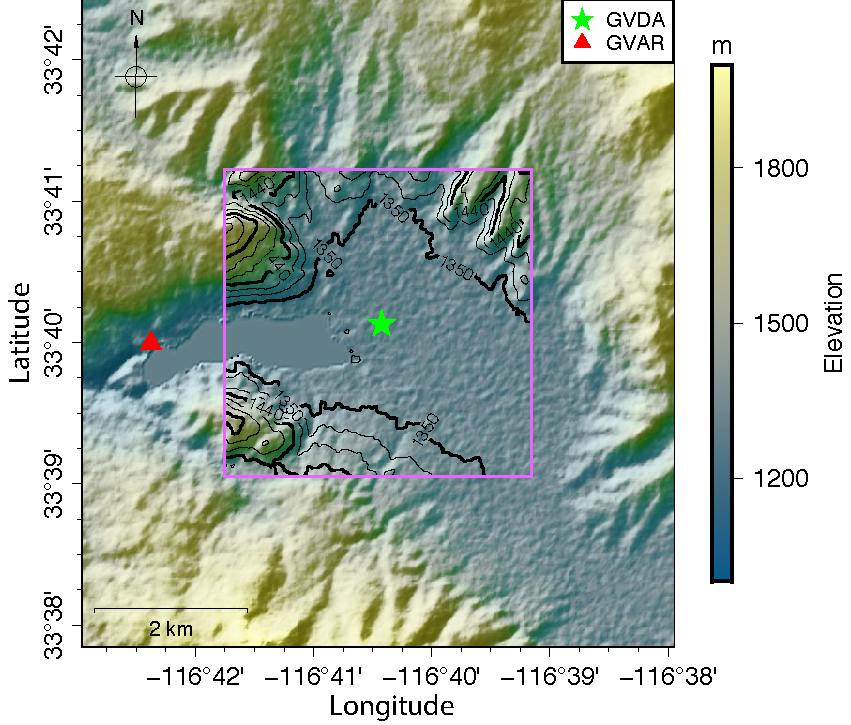
\includegraphics[width=0.9\textwidth]{figures/figure_etf_1.pdf}
  \caption{Site map of Garner Valley Downhole Array (GVDA), denoted by the star. The rectangle depicts the extent of the modeling domain, where the contours depict elevation in meters. The triangle denotes a nearby outcrop site GVAR. The color version of this figure is available only in the electronic edition.}
  \label{fig:etf-1}
\end{figure}

\clearpage
\begin{figure}[!ht]
  \centering
  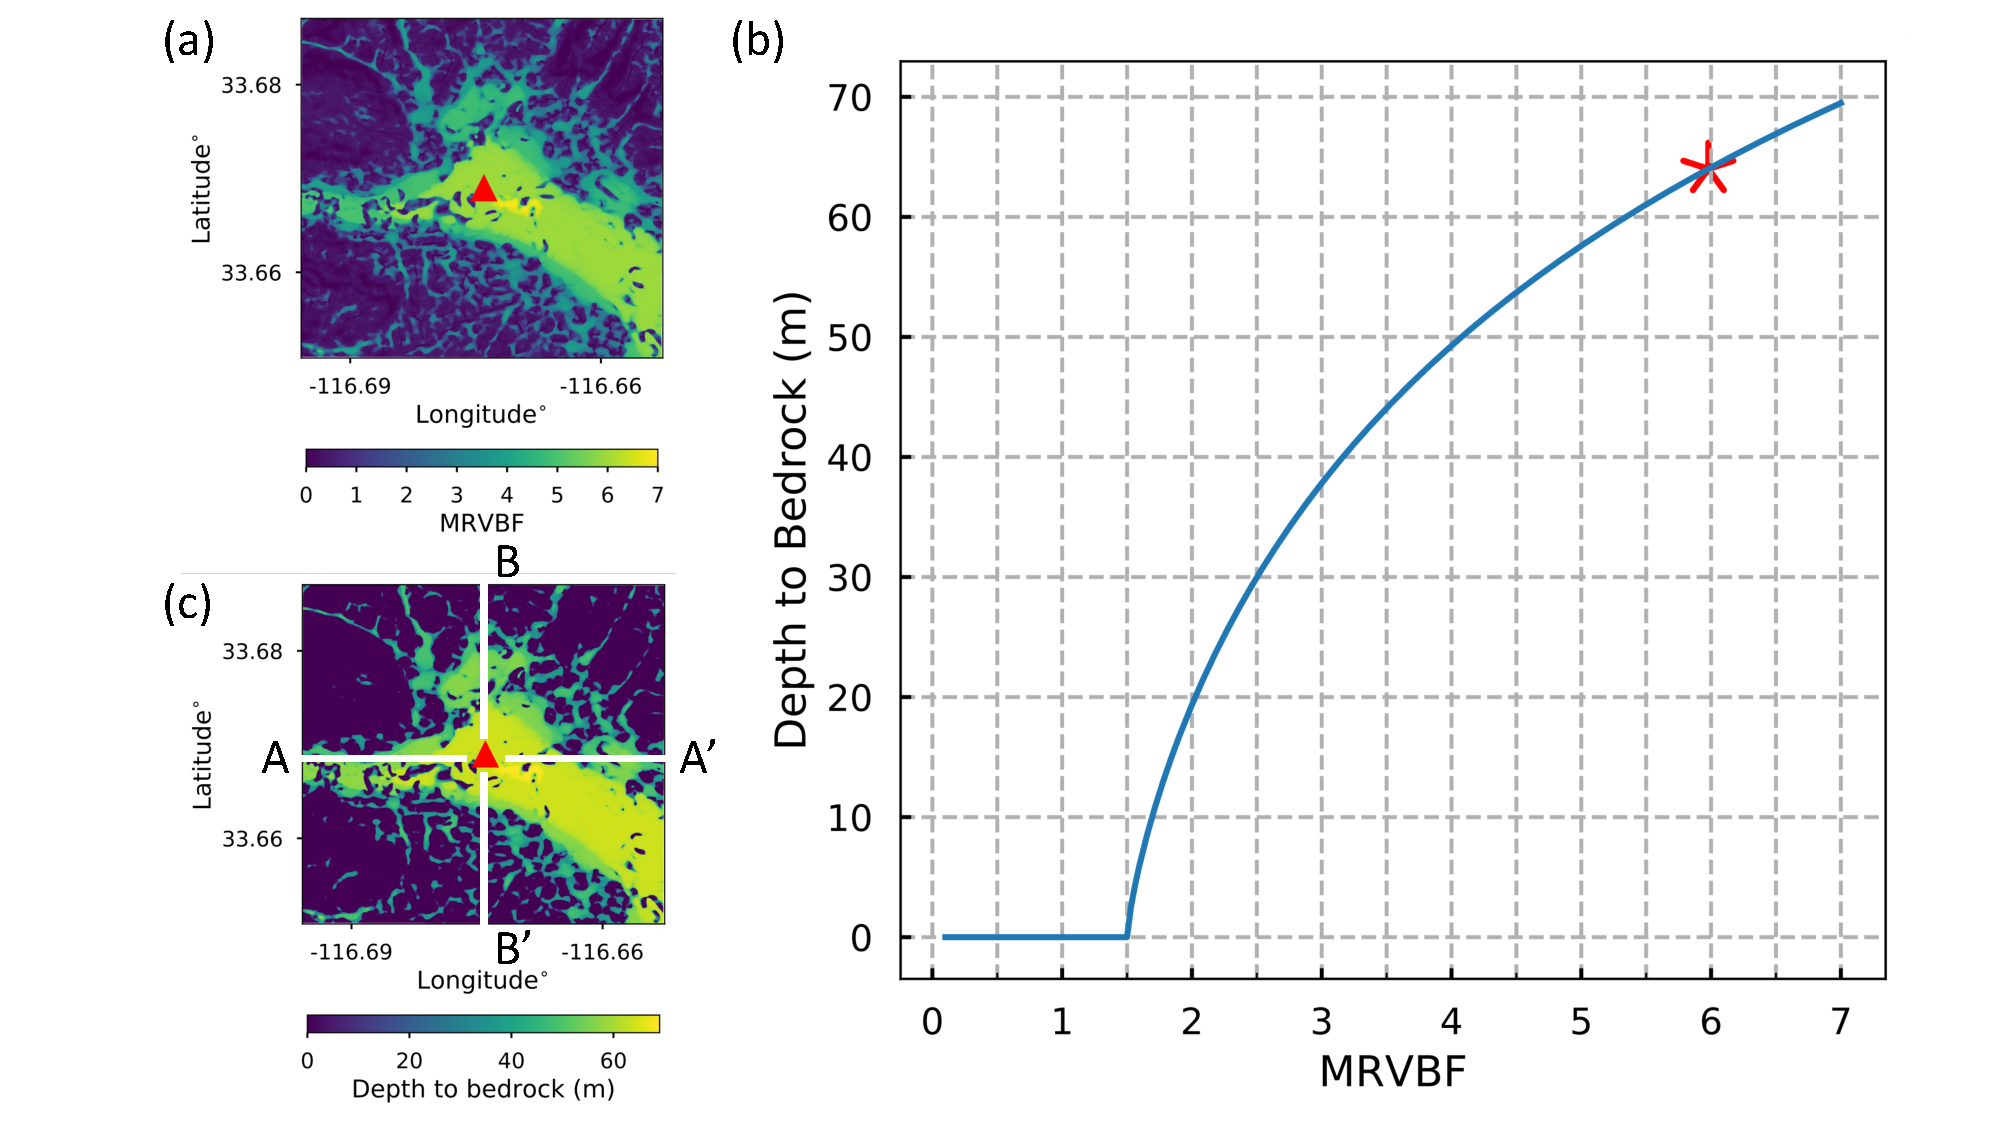
\includegraphics[width=0.9\textwidth]{figures/figure_etf_2.pdf}
  \caption{(a) Multiresolution index of valley bottom flatness (MRVBF) and (b) the bedrock depth map surrounding GVDA, which is depicted by a triangle in both figures. (c) The mapping function from MRVBF to bedrock depth, with GVDA marked with an asterisk. The color version of this figure is available only in the electronic edition.}
  \label{fig:etf-2}
\end{figure}

\clearpage
\begin{figure}[!ht]
  \centering
  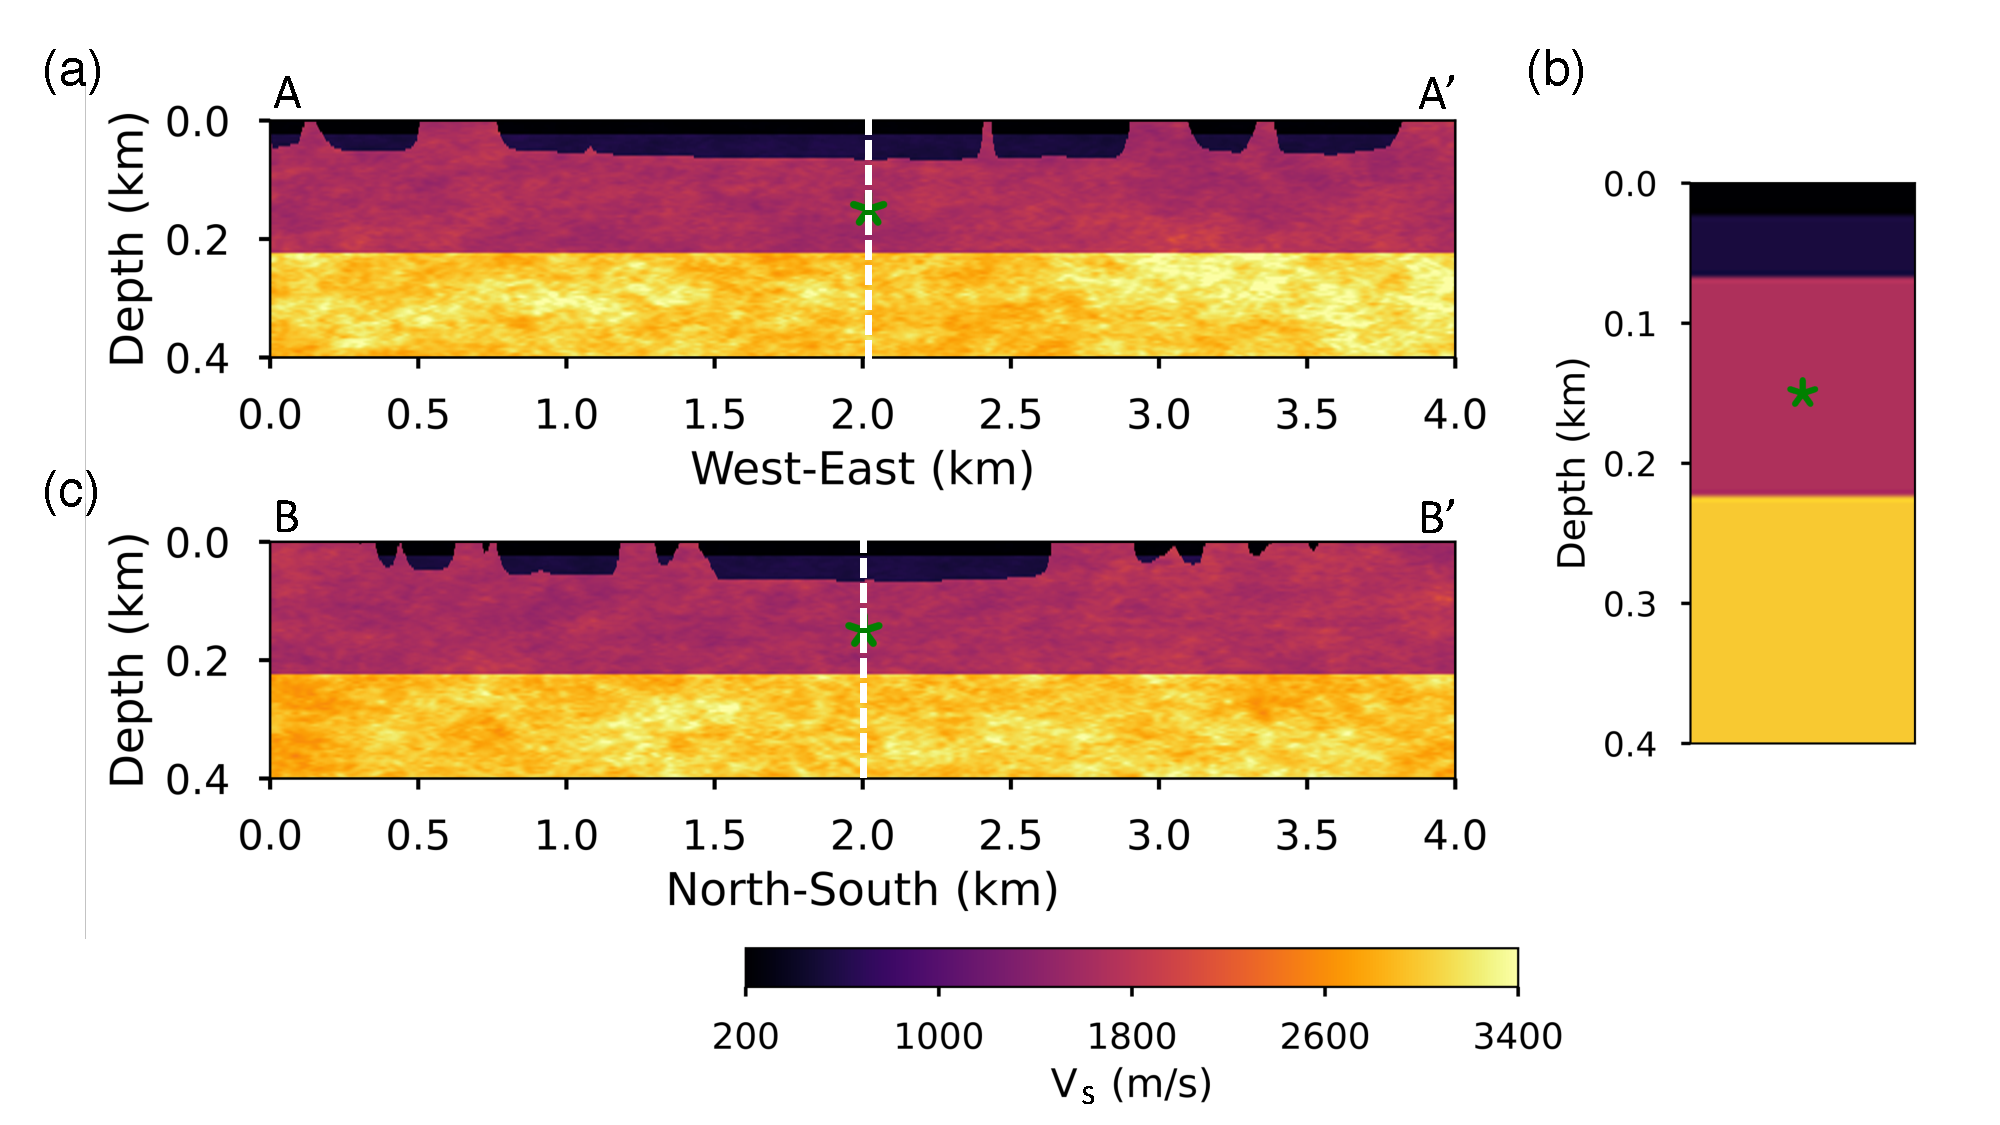
\includegraphics[width=0.9\textwidth]{figures/figure_etf_3.pdf}
  \caption{Cross sections of $V_S$ in the 3D mesh (see \cref{fig:etf-2}) intersecting GVDA along (a) A–A' and (c) B–B'; the downhole accelerometer is denoted with the asterisk. (b) The 1D $V_S$ profile, with its location denoted by the dashed line in the left panels, obtained from the borehole log, and used in the SH1D model. The color version of this figure is available only in the electronic edition.}
  \label{fig:etf-3}
\end{figure}

\clearpage
\begin{figure}[!ht]
  \centering
  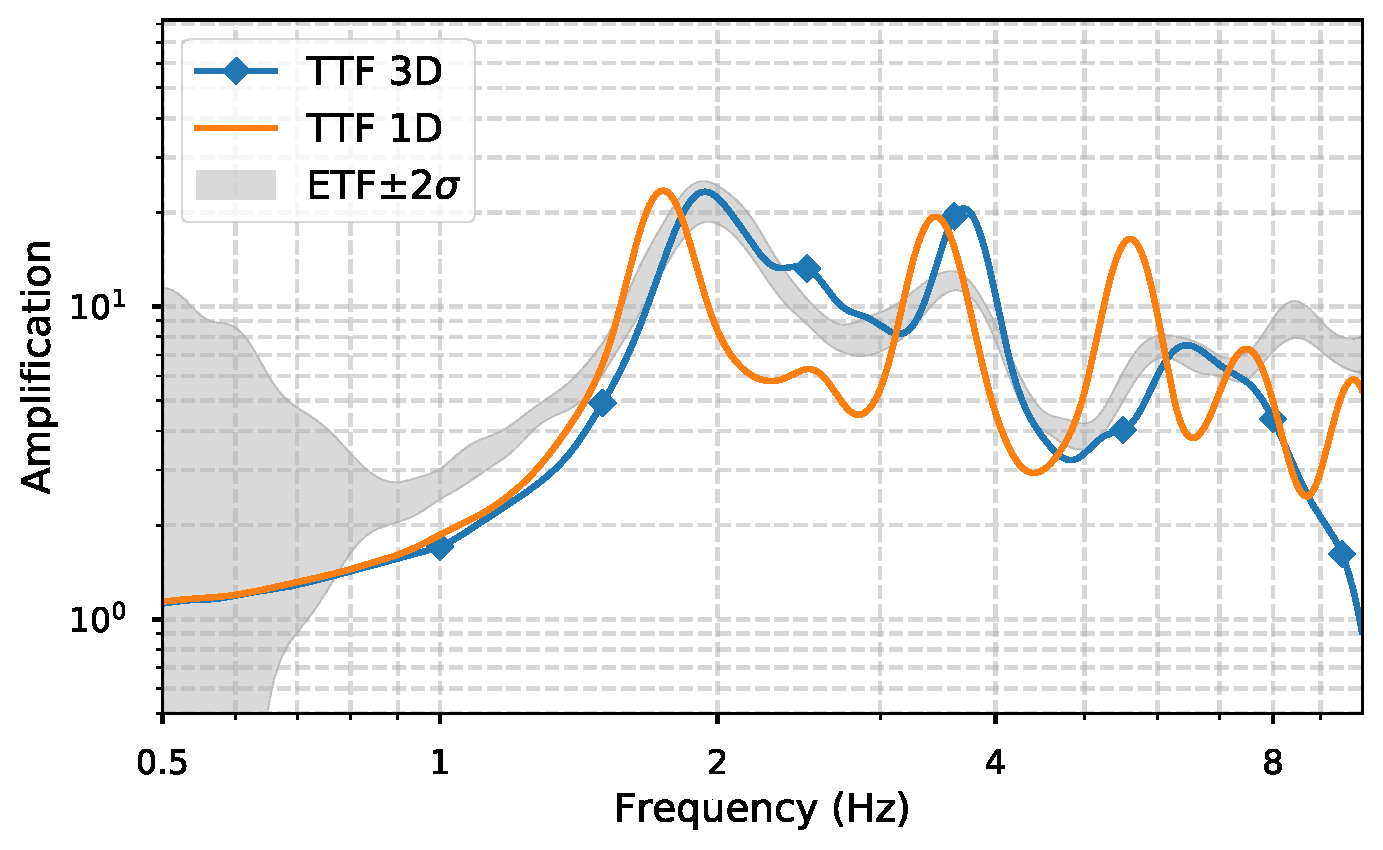
\includegraphics[width=0.9\textwidth]{figures/figure_etf_4.pdf}
  \caption{Comparison between the theoretical transfer functions (TTFs) computed using the 3D model and the SH1D model at GVDA, with the two-sigma scatter of empirical transfer functions (ETFs) shaded in gray. The color version of this figure is available only in the electronic edition.}
  \label{fig:etf-4}
\end{figure}

\clearpage
\begin{figure}[!ht]
  \centering
  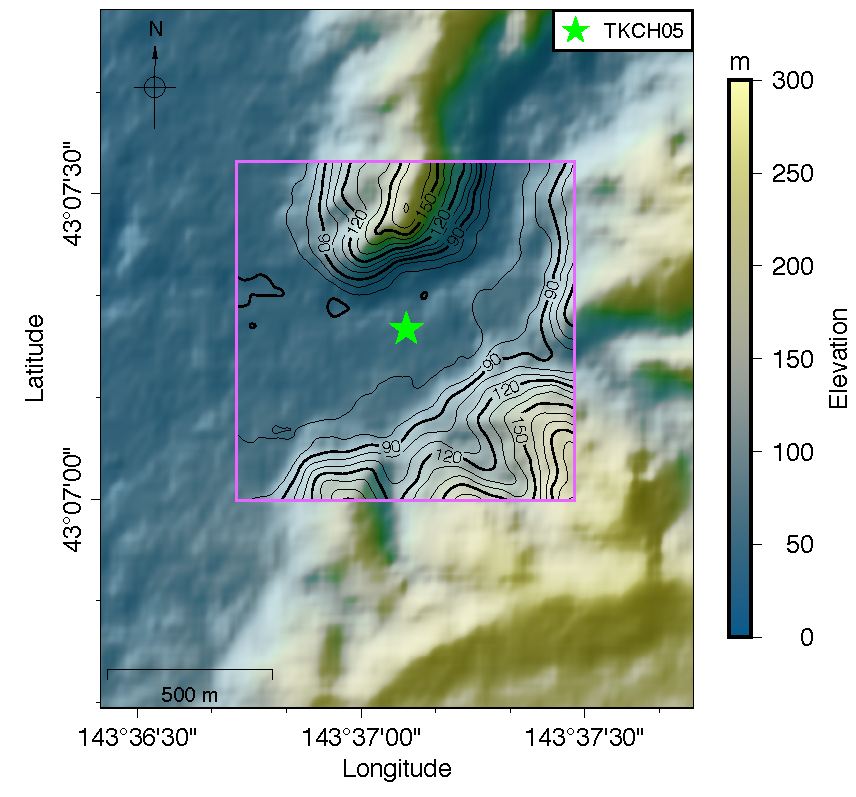
\includegraphics[width=0.9\textwidth]{figures/figure_etf_5.pdf}
  \caption{Site map of TKCH05, denoted by the star. The rectangle depicts the extent of the modeling domain, where the contours depict elevation in meters. The color version of this figure is available only in the electronic edition.}
  \label{fig:etf-5}
\end{figure}

\clearpage
\begin{figure}[!ht]
  \centering
  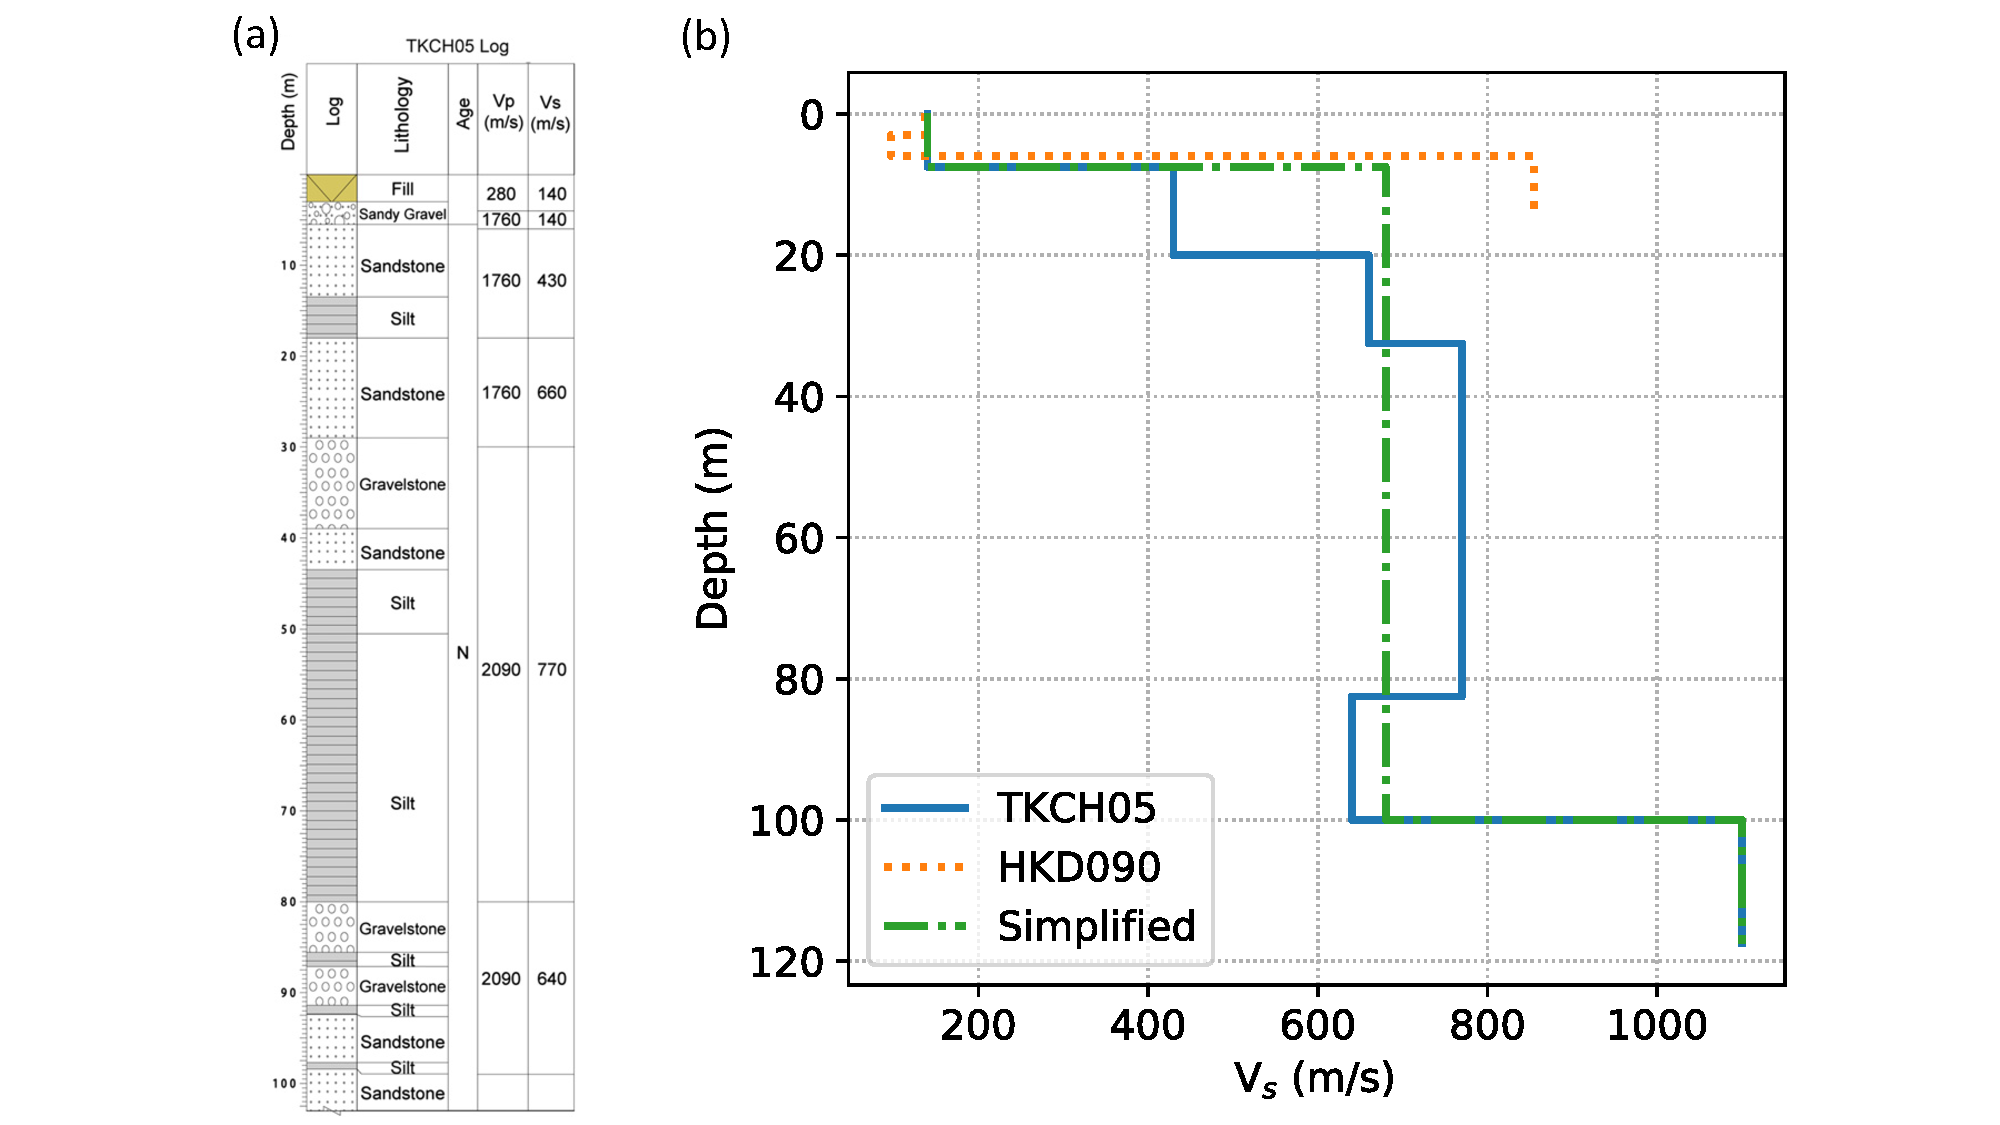
\includegraphics[width=0.9\textwidth]{figures/figure_etf_6.pdf}
  \caption{(a) Borehole log at TKCH05 (from \citealt{thompsonTaxonomySiteResponse2012}). (b) Borehole $V_S$ profiles at TKCH05 and HKD090, as well as for our simplified 1D model. The color version of this figure is available only in the electronic edition.}
  \label{fig:etf-6}
\end{figure}

\clearpage
\begin{figure}[!ht]
  \centering
  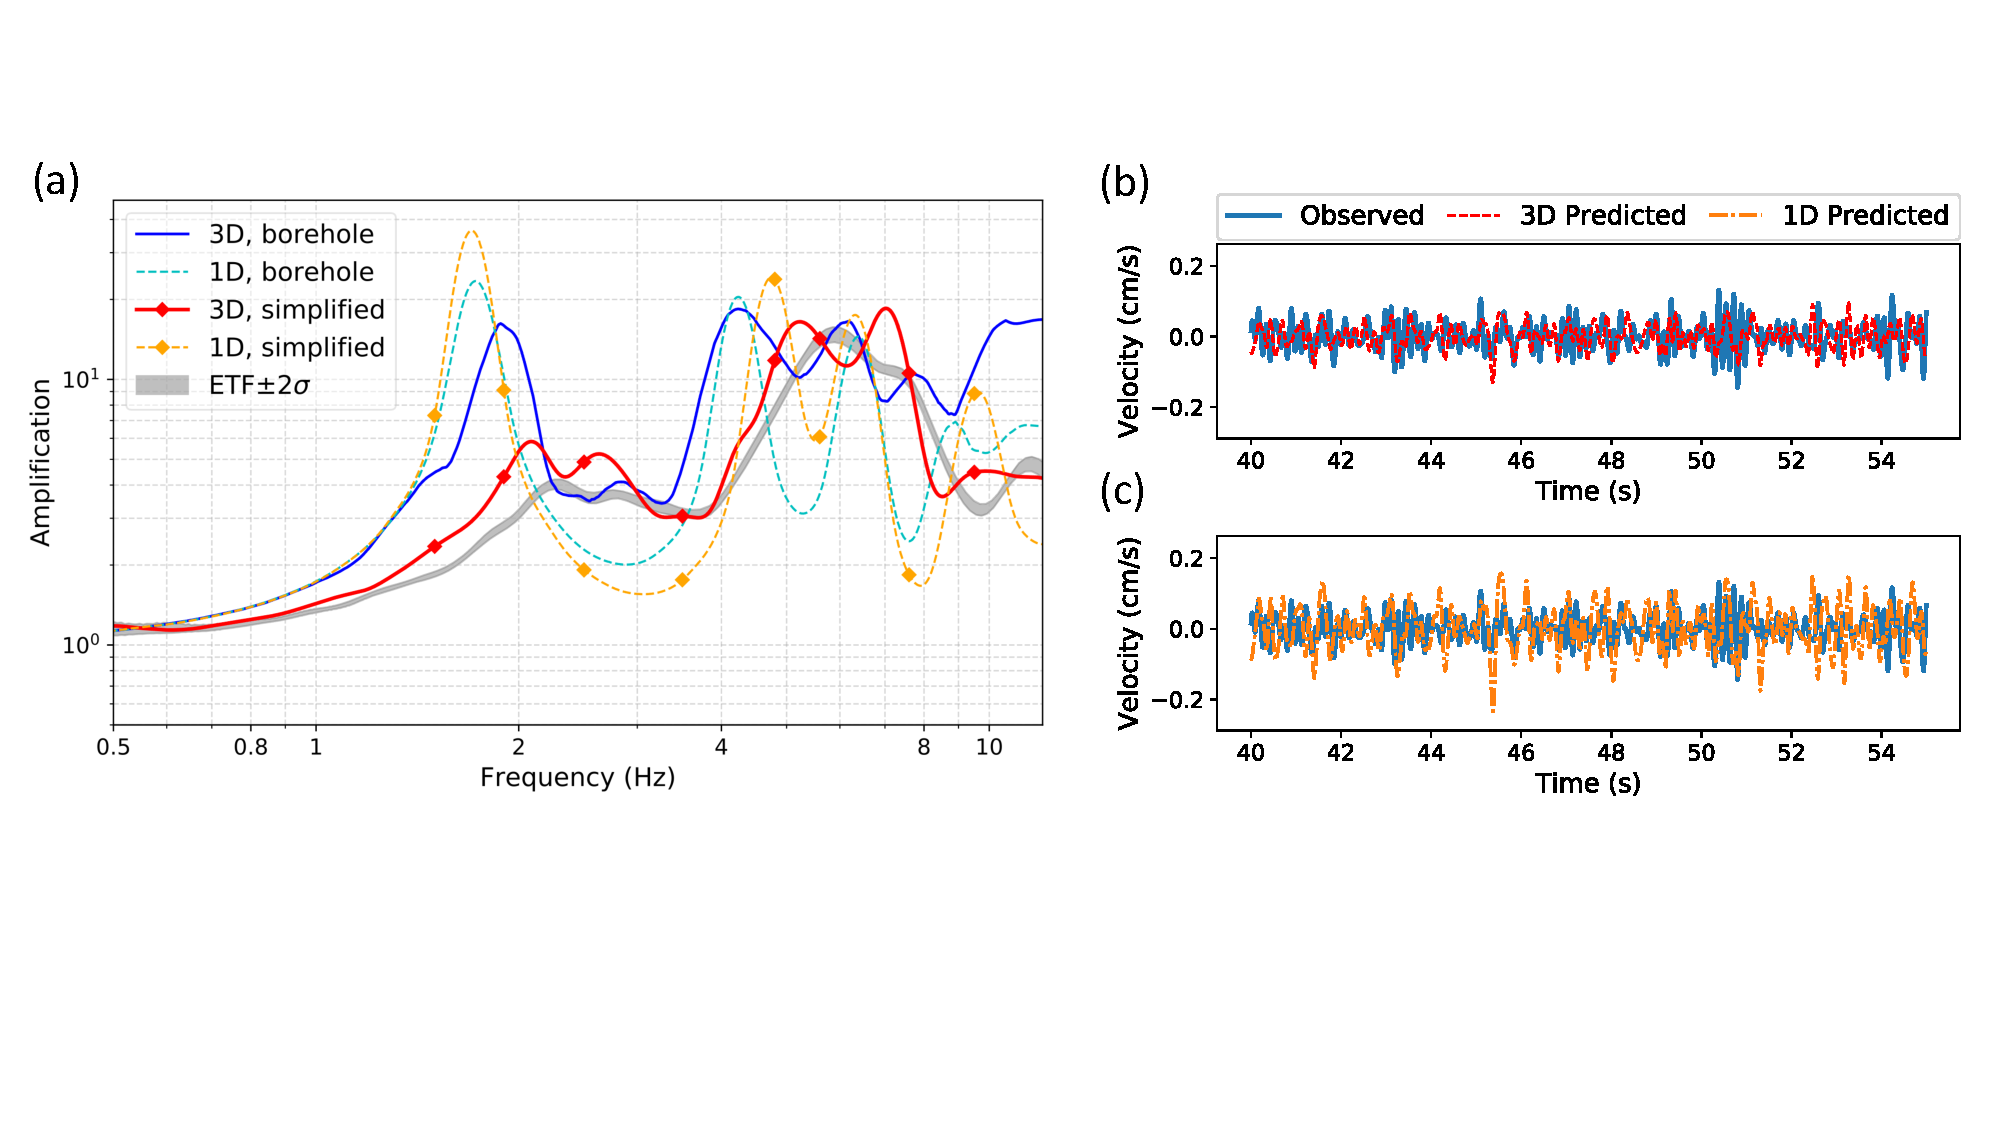
\includegraphics[width=0.9\textwidth]{figures/figure_etf_7.pdf}
  \caption{(a) Comparison between TTFs and the two-sigma scatter of the ETF for 3D and 1D models at TKCH05. Solid and dashed lines without markers are the 3D and 1D models based on the borehole log profile, respectively; solid and dashed lines with diamond markers depict the 3D and 1D models, based on the simplified downhole profile. (b,c) Comparison of 1.5–8 Hz observed east–west component surface ground motions with those obtained from convolution of the downhole records with the TTFs from models using the simplified profile for the (b) 3D model and (c) 1D model. The color version of this figure is available only in the electronic edition.}
  \label{fig:etf-7}
\end{figure}

\clearpage
\begin{figure}[!ht]
  \centering
  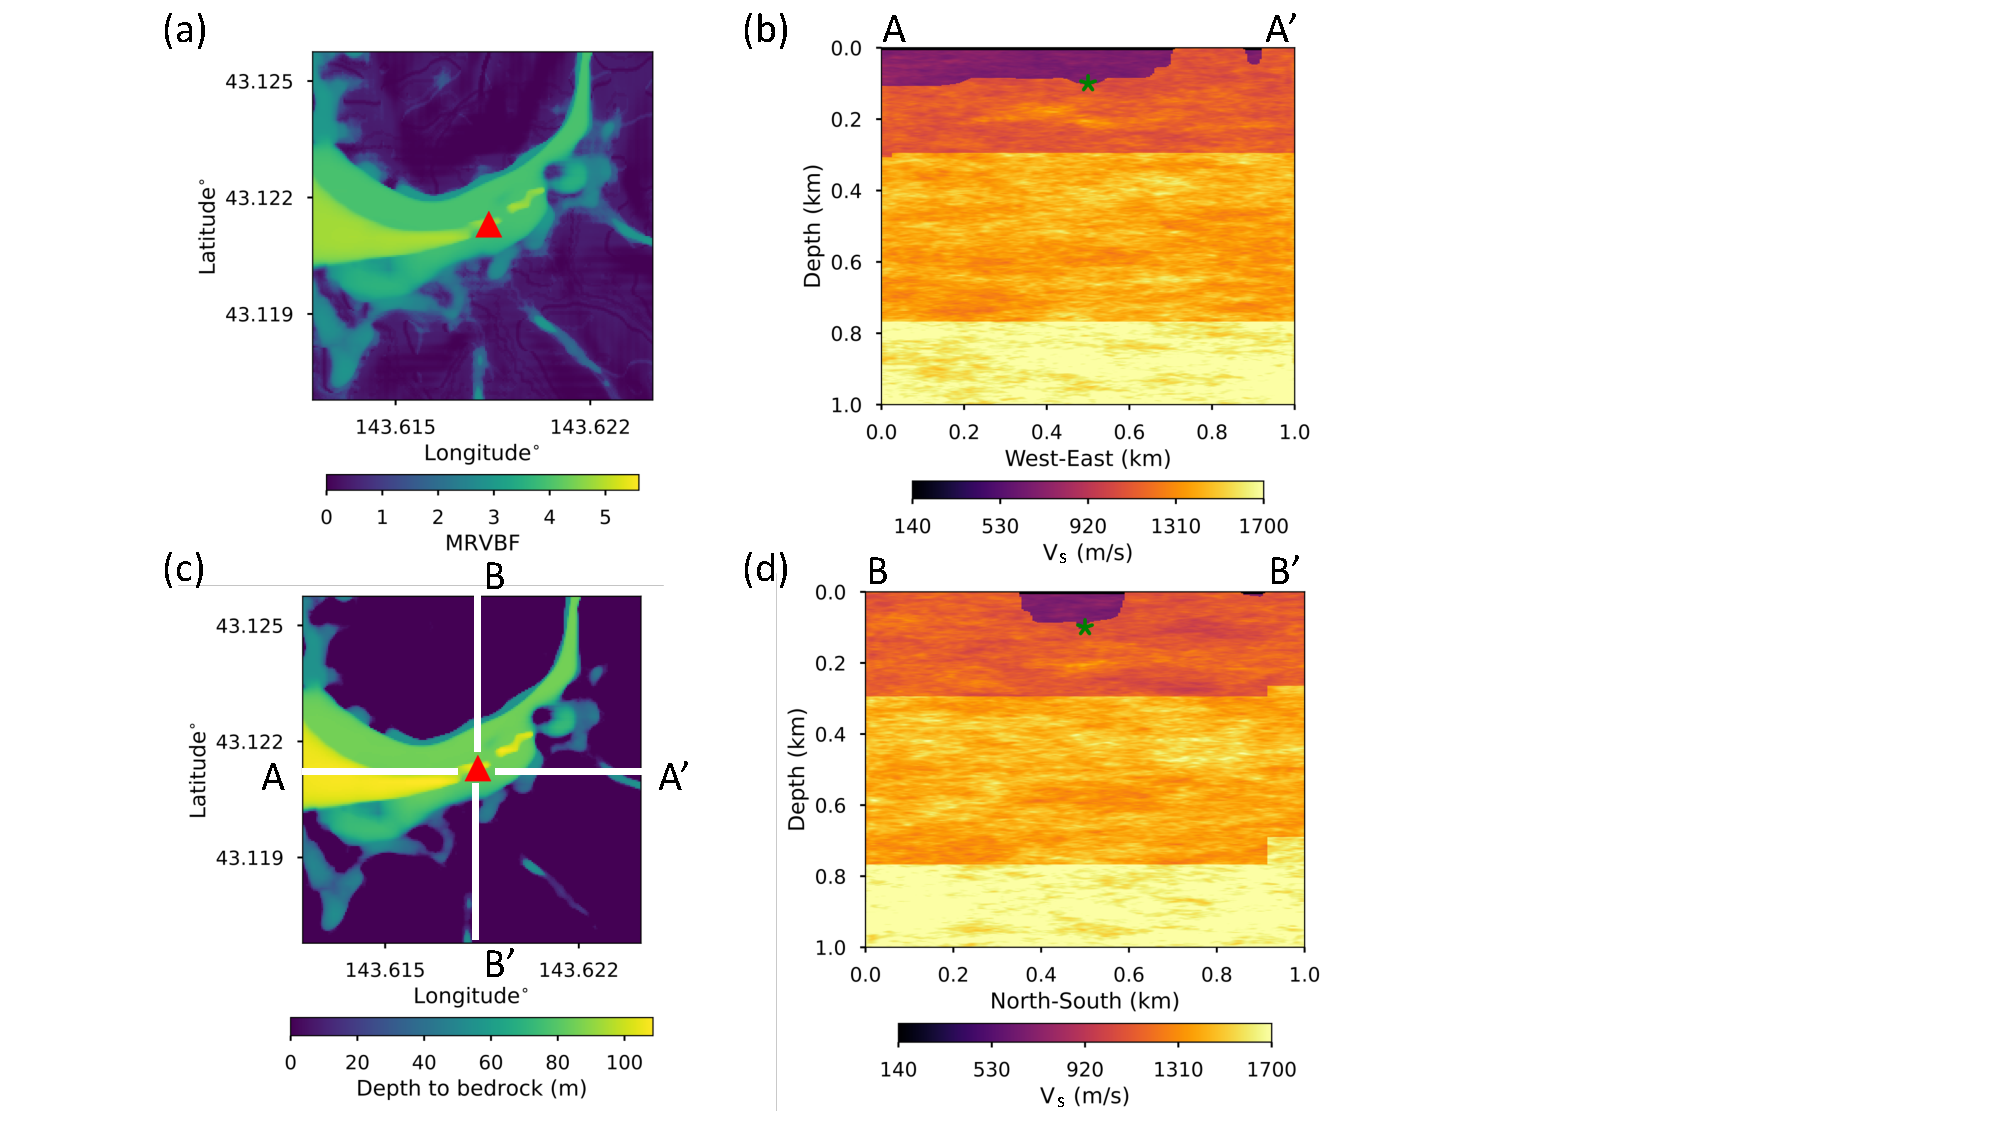
\includegraphics[width=0.9\textwidth]{figures/figure_etf_8.pdf}
  \caption{(a) MRVBF and (c) depth to bedrock in the vicinity of TKCH05, with the site location denoted by the triangle. (b) West–east A–A' and (d) north–south B–B' cross sections intersecting TKCH05, the downhole sensor is marked with the asterisk. The color version of this figure is available only in the electronic edition.}
  \label{fig:etf-8}
\end{figure}

\clearpage
\begin{figure}[!ht]
  \centering
  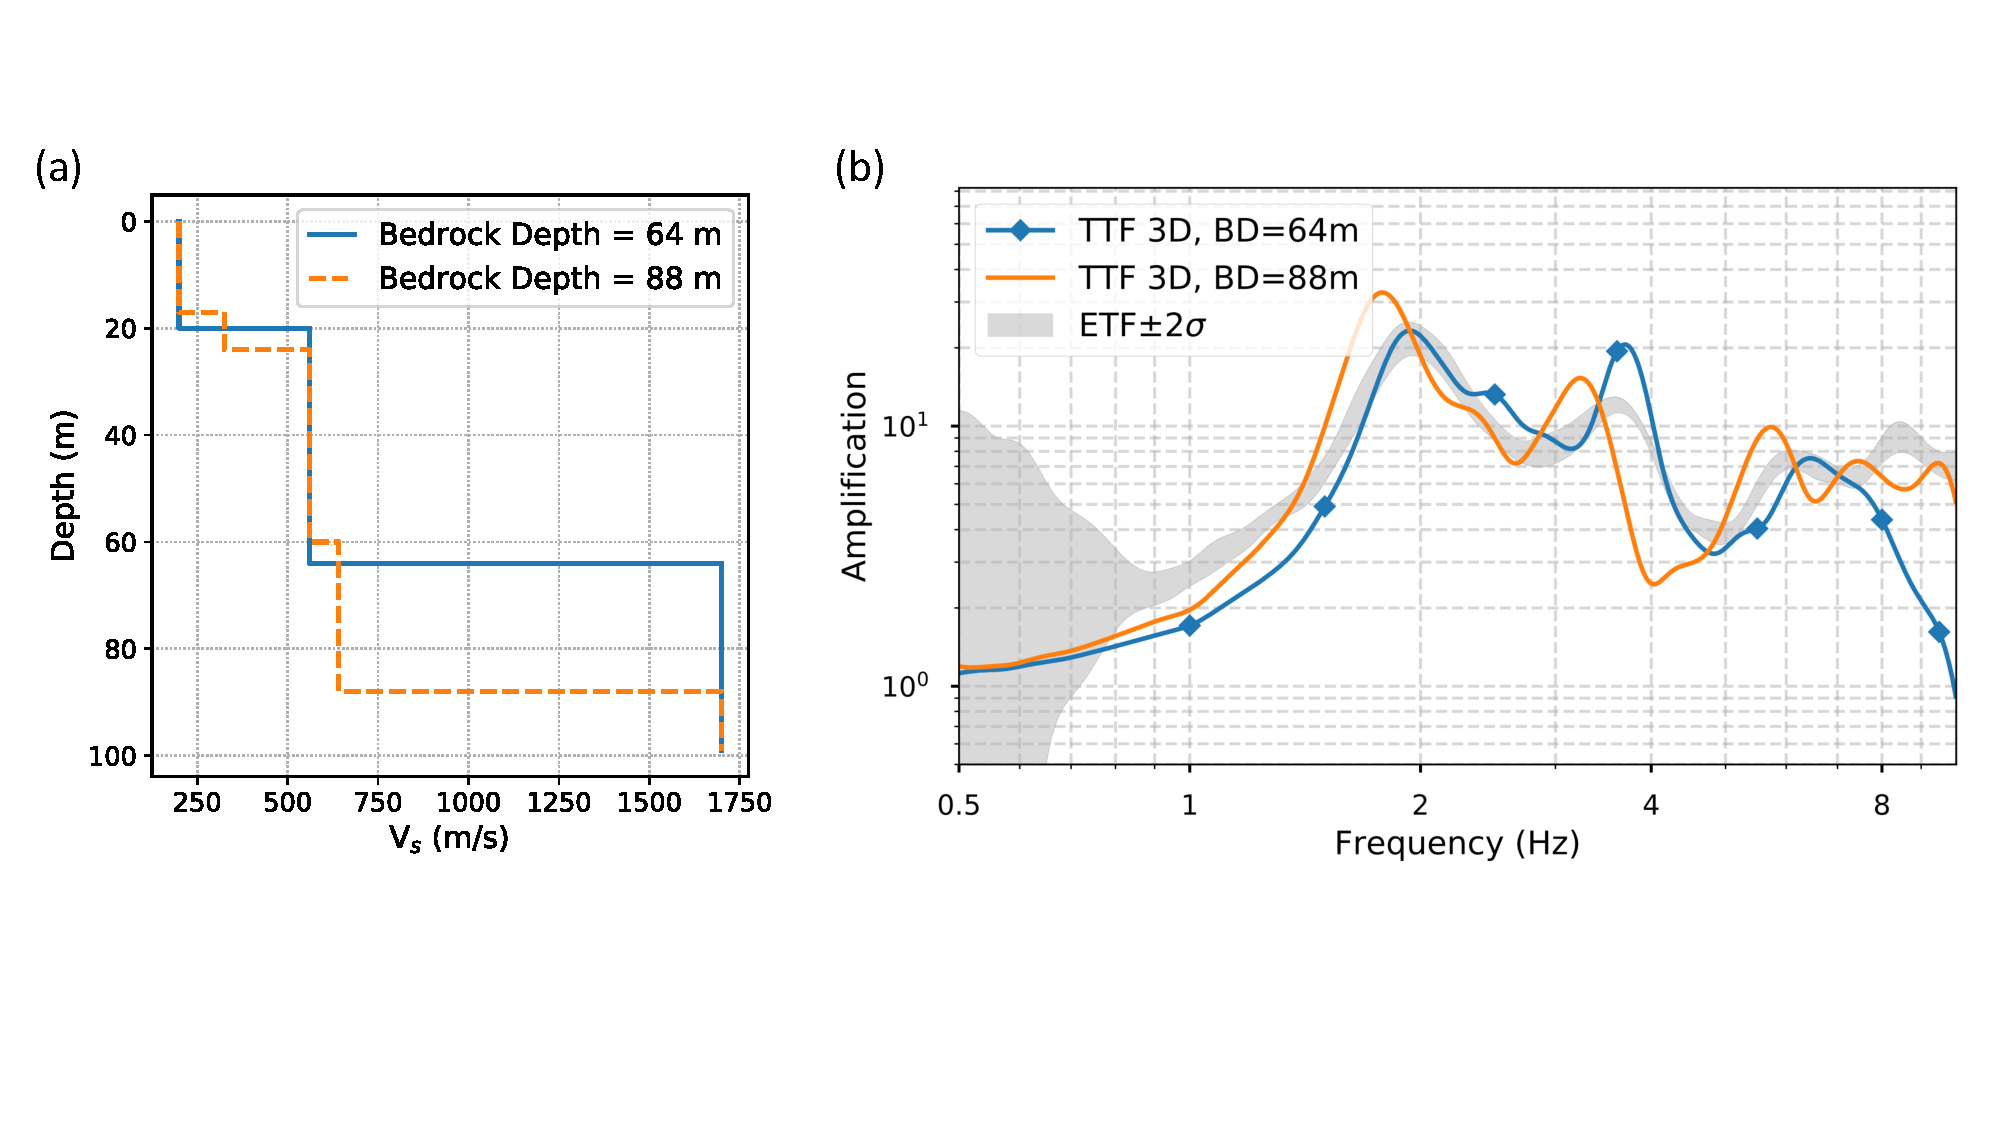
\includegraphics[width=0.9\textwidth]{figures/figure_etf_9.pdf}
  \caption{(a) The Gibbs and Steller velocity profiles at GVDA, in which the bedrock depth is 64 (solid line) and 88 m (dashed line), respectively. (b) Comparison between the two-sigma scatter of the ETFs (gray shaded) and the TTFs from the 3D models assembled with the Gibbs and Steller profiles, respectively. The color version of this figure is available only in the electronic edition.}
  \label{fig:etf-9}
\end{figure}

\clearpage
\begin{figure}[!ht]
  \centering
  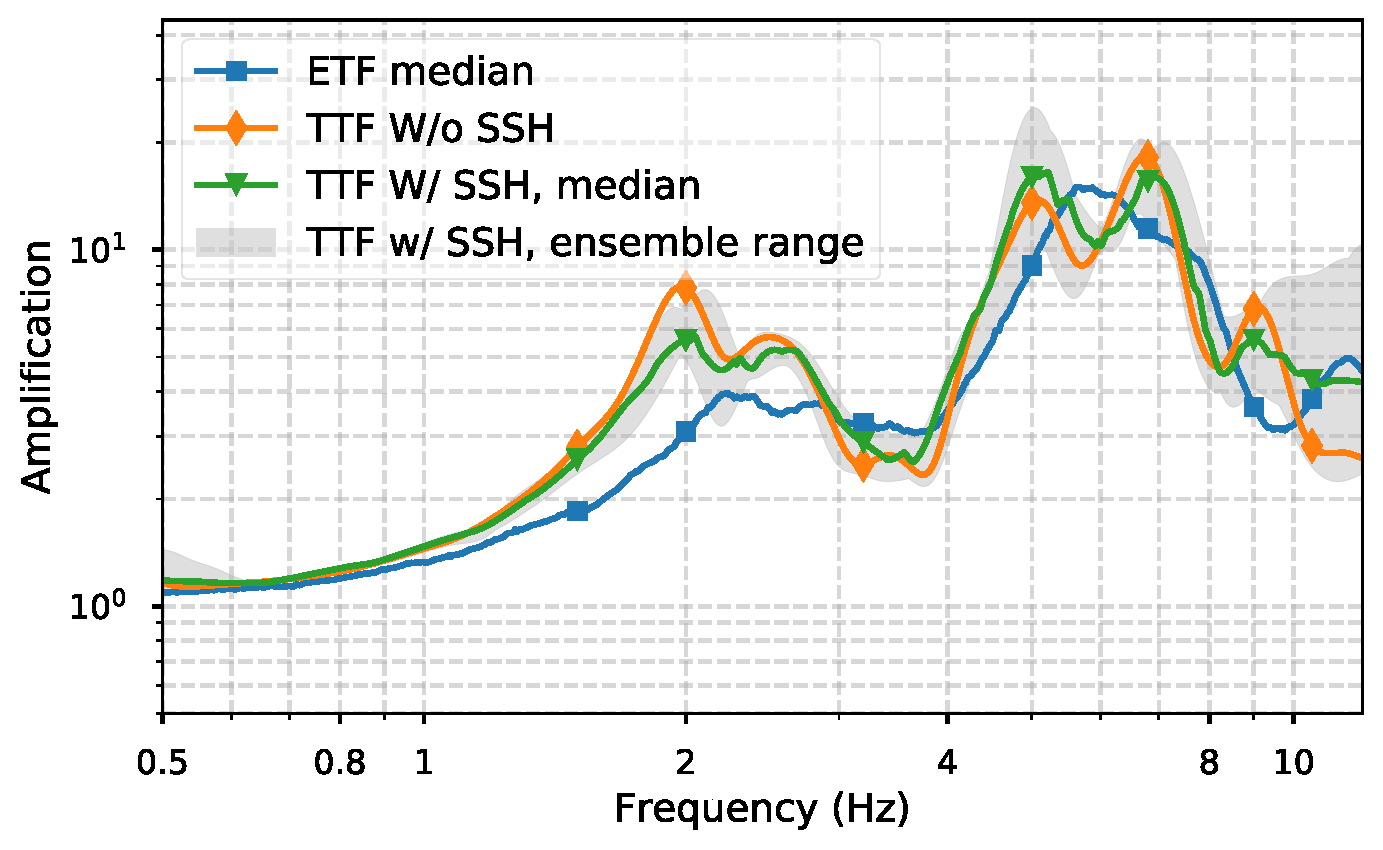
\includegraphics[width=0.9\textwidth]{figures/figure_etf_10.pdf}
  \caption{Comparison between the median ensemble ETF, the TTF from the 3D model without and with small-scale heterogeneities (SSHs) at TKCH05. The gray shaded region is the range of maximum and minimum values encountered in TTFs from these realizations of SSHs. The color version of this figure is available only in the electronic edition.}
  \label{fig:etf-10}
\end{figure}

\clearpage
\begin{figure}[!ht]
  \centering
  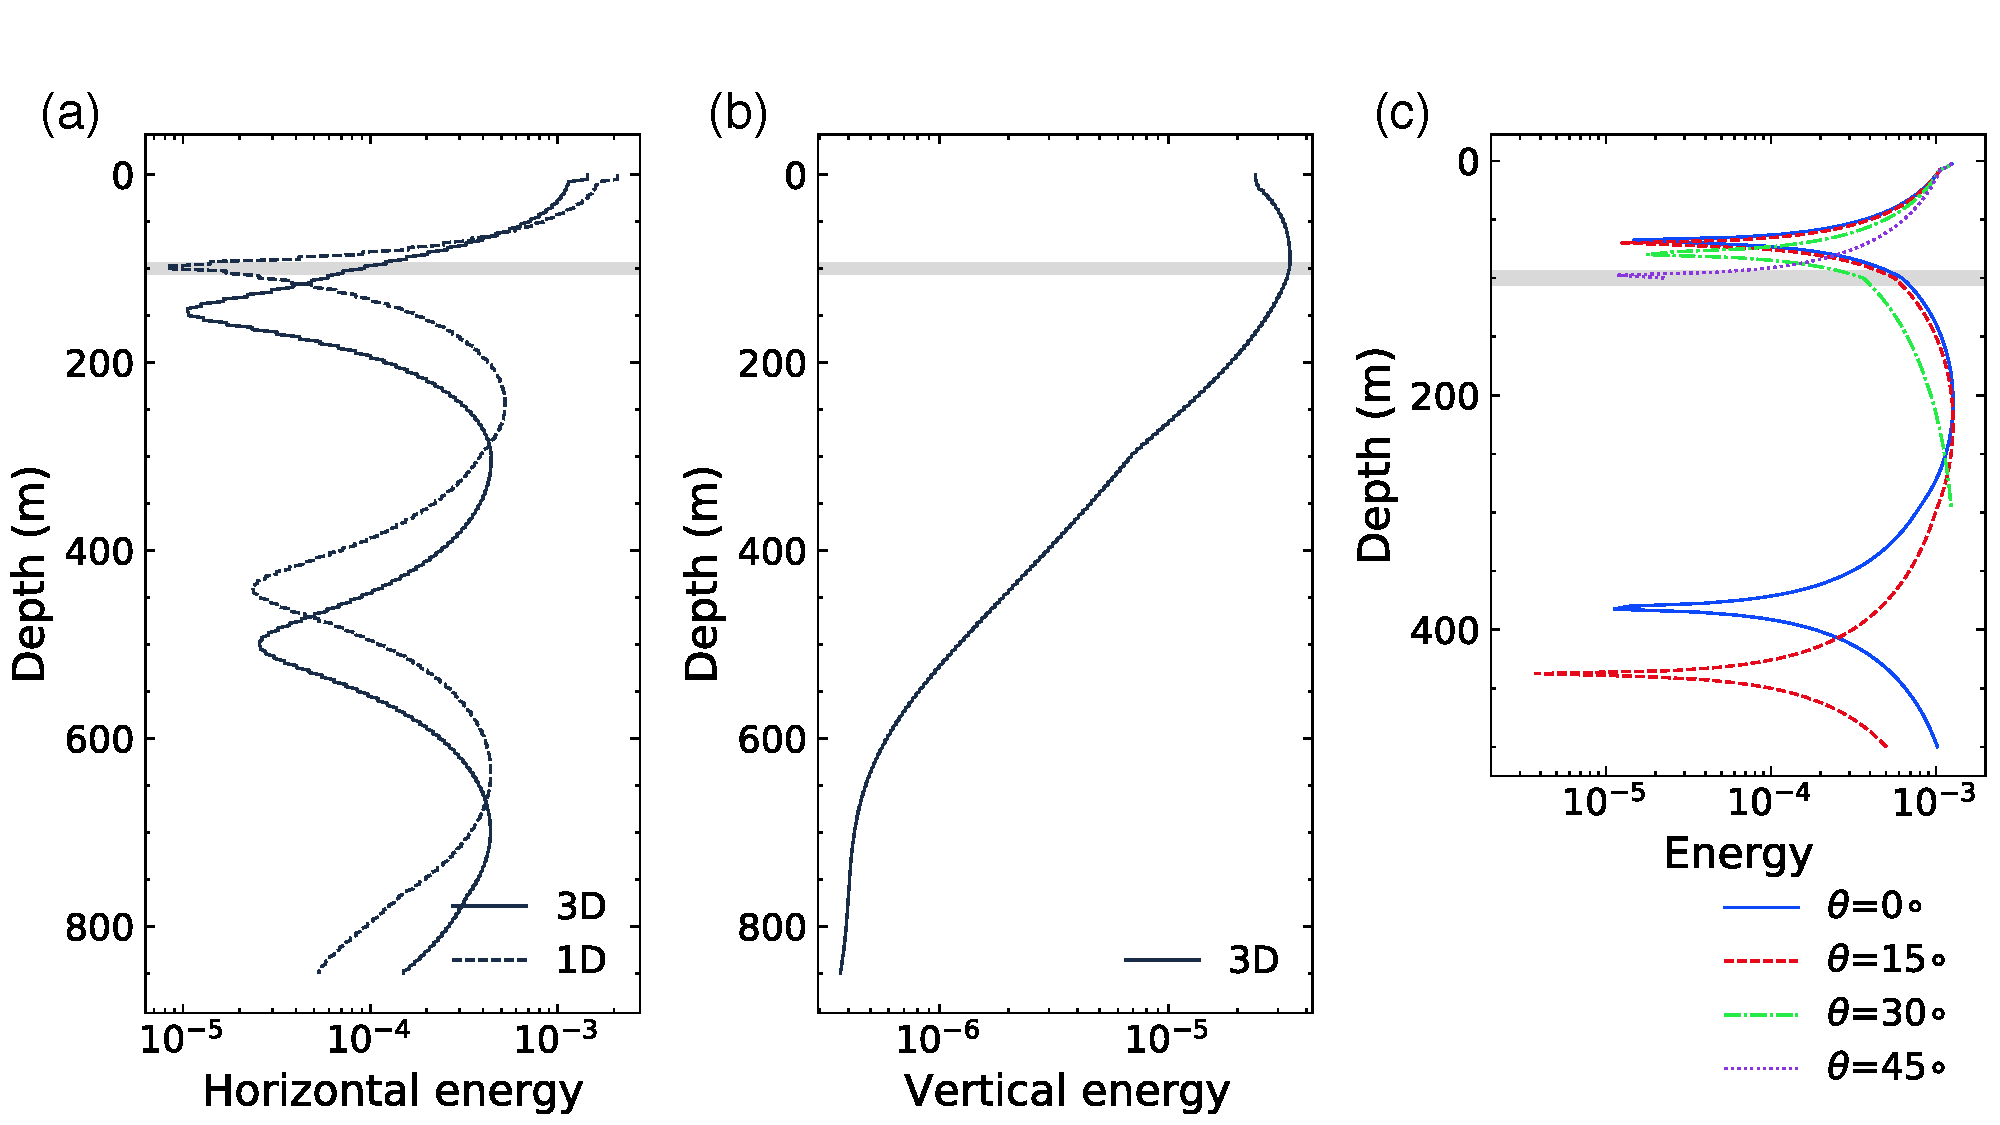
\includegraphics[width=0.9\textwidth]{figures/figure_etf_11.pdf}
  \caption{Energy on the (a) horizontal and (b) vertical components at the site TKCH05. (c) Total energy along depth using the simplified velocity profile at TKCH05 with different incidence angles. The gray horizontal line, at around 100 m depth, depicts the downhole site depth. The color version of this figure is available only in the electronic edition.}
  \label{fig:etf-11}
\end{figure}


%% supplement
\setcounter{table}{0}
\setcounter{figure}{0}
\numberwithin{figure}{chapter}
\numberwithin{table}{chapter}
\renewcommand{\thetable}{S\arabic{chapter}.\arabic{table}}
\renewcommand{\thefigure}{S\arabic{chapter}.\arabic{figure}}
\newpage
\section*{Supplementary Materials}
\addcontentsline{toc}{section}{\protect\numberline{}Supplementary Materials}

This supplement includes one figure (\Cref{fig:etf-S1}) showing the location of the events used in the GVDA study and recorded accelerations at a subset of events, one figure (\Cref{fig:etf-S2}) showing the locations of the events used in the TKCH05 study and recorded accelerations at a subset of events, and two figures (\Cref{fig:etf-S3,fig:etf-S4}) showing the comparison of snapshots generated in 3D and 1D models at the TKCH05 site in Japan.

\clearpage
\floatsetup[figure]{style=plain,subcapbesideposition=top}
\begin{figure}[!ht]
  \sidesubfloat[]{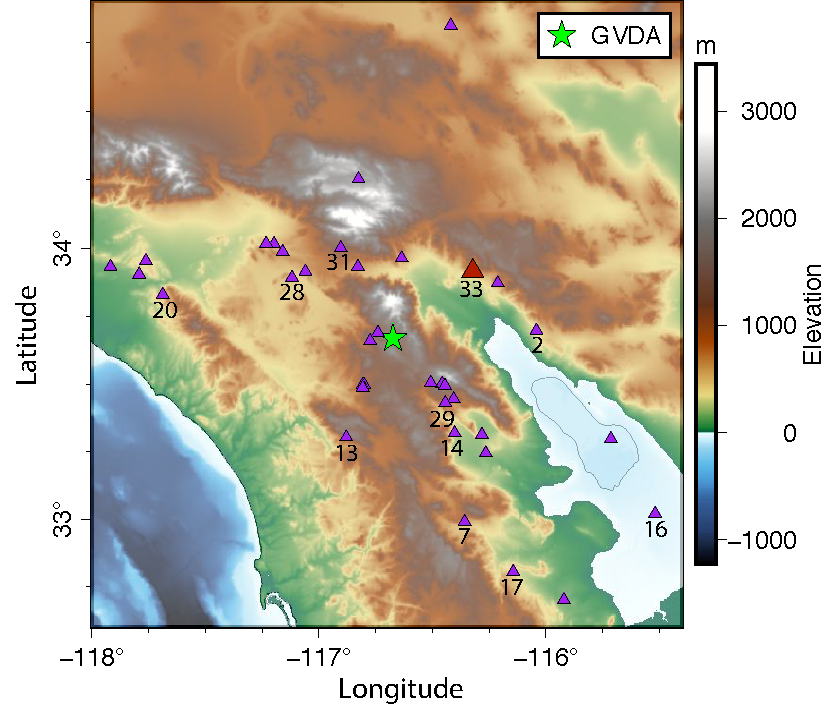
\includegraphics[width=0.31\textwidth]{figures/figure_etf_S1a.pdf}\label{fig:etf-S1a}} \hfil
  \sidesubfloat[]{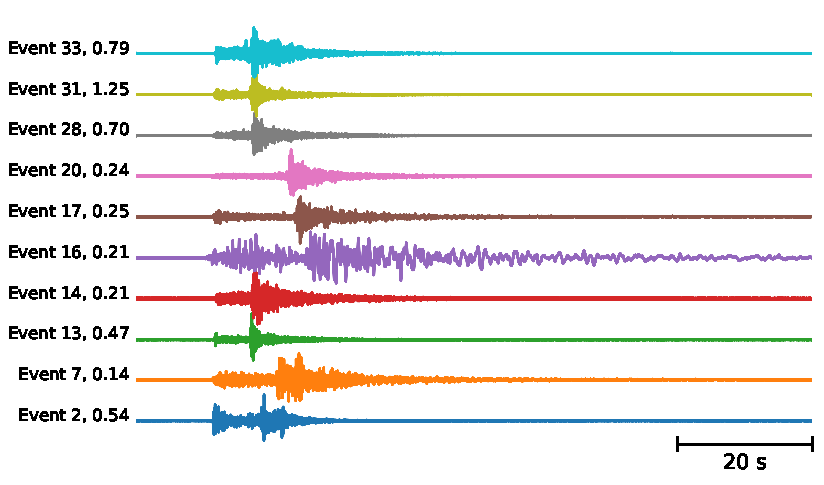
\includegraphics[width=0.45\textwidth]{figures/figure_etf_S1b.pdf}\label{fig:etf-S1b}} % \\[\baselineskip]%
  \caption{(a) Map of events (purple triangles) used for computing the ETFs at GVDA. The red triangle depicts the event used in simulations. (b) Recorded accelerations (normalized) along West-East direction at 10 randomly selected sites. The maximum amplitude is showed to the left of each line.}
  \label{fig:etf-S1}
\end{figure}


\clearpage
\floatsetup[figure]{style=plain,subcapbesideposition=top}
\begin{figure}[!ht]
  \sidesubfloat[]{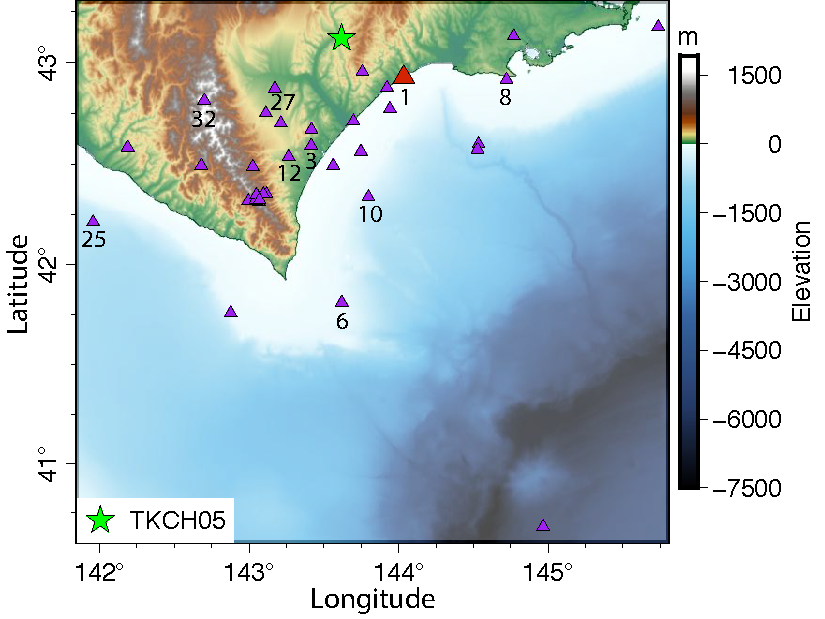
\includegraphics[width=0.33\textwidth]{figures/figure_etf_S2a.pdf}\label{fig:etf-S2a}} \hfil
  \sidesubfloat[]{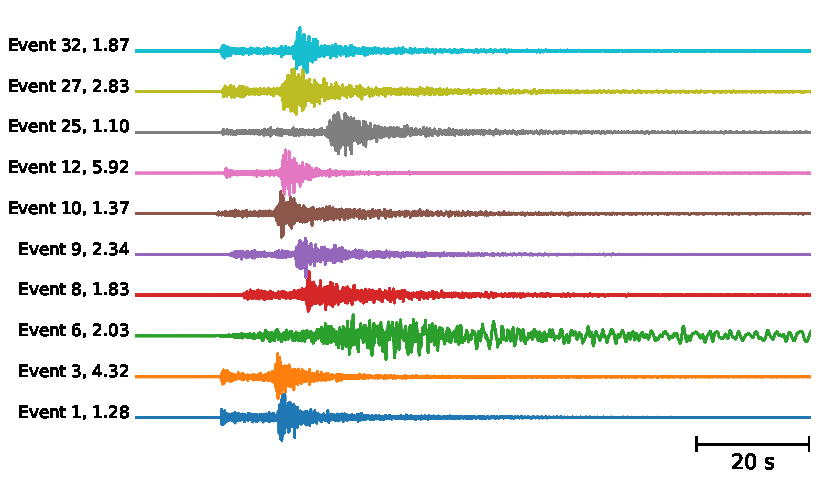
\includegraphics[width=0.42\textwidth]{figures/figure_etf_S2b.pdf}\label{fig:etf-S2b}} % \\[\baselineskip]%
  \caption{(a) Map of events (purple triangles) used for computing the ETFs at TKCH05. The red triangle depicts the event used in simulations. (b) Recorded accelerations (normalized) along West-East direction at 10 randomly selected sites. The maximum amplitude is showed to the left of each line.}
  \label{fig:etf-S2}
\end{figure}


\clearpage
\floatsetup[figure]{style=plain,subcapbesideposition=top}
\begin{figure}[!ht]
  \sidesubfloat[]{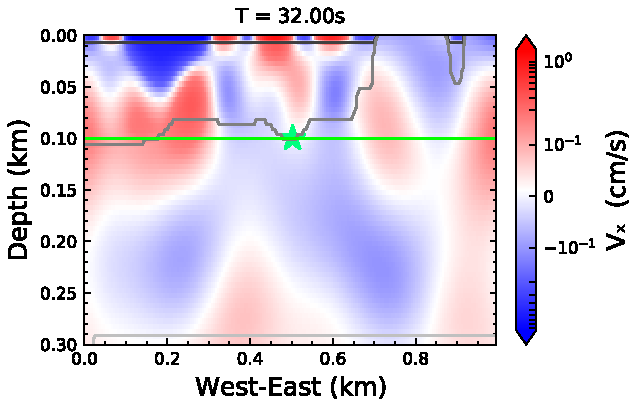
\includegraphics[width=0.4\textwidth]{figures/figure_etf_S3a.pdf}\label{fig:etf-S3a}} \hfil
  \sidesubfloat[]{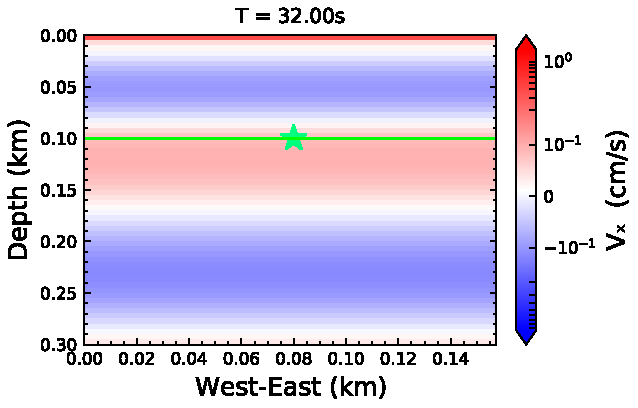
\includegraphics[width=0.4\textwidth]{figures/figure_etf_S3b.pdf}\label{fig:etf-S3b}} \\[\baselineskip]%
  \sidesubfloat[]{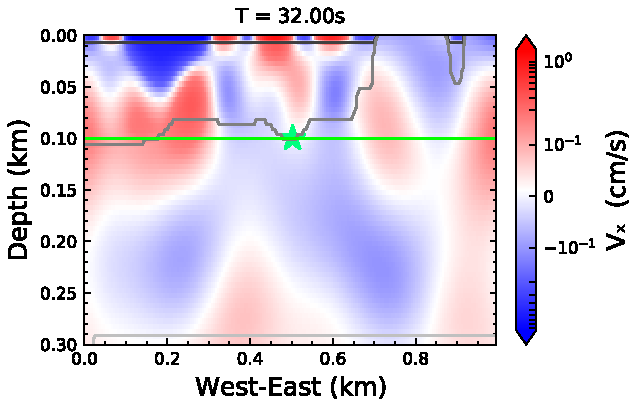
\includegraphics[width=0.4\textwidth]{figures/figure_etf_S3a.pdf}\label{fig:etf-S3c}} \hfil
  \sidesubfloat[]{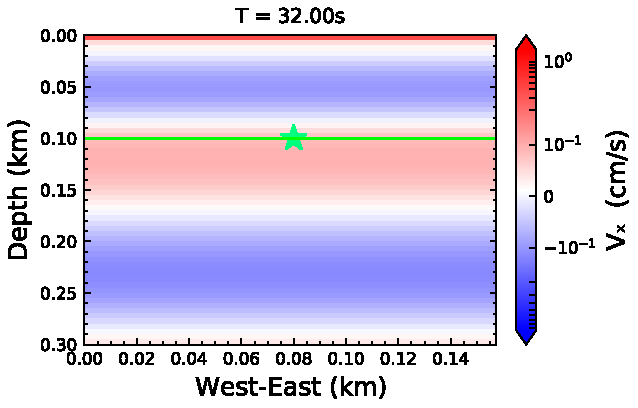
\includegraphics[width=0.4\textwidth]{figures/figure_etf_S3b.pdf}\label{fig:etf-S3d}} \\[\baselineskip]%
  \sidesubfloat[]{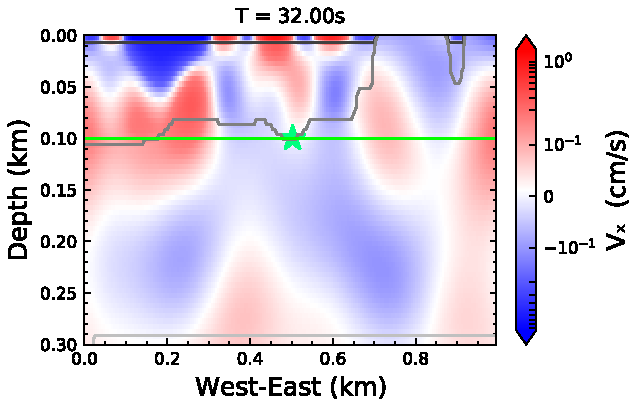
\includegraphics[width=0.4\textwidth]{figures/figure_etf_S3a.pdf}\label{fig:etf-S3e}} \hfil
  \sidesubfloat[]{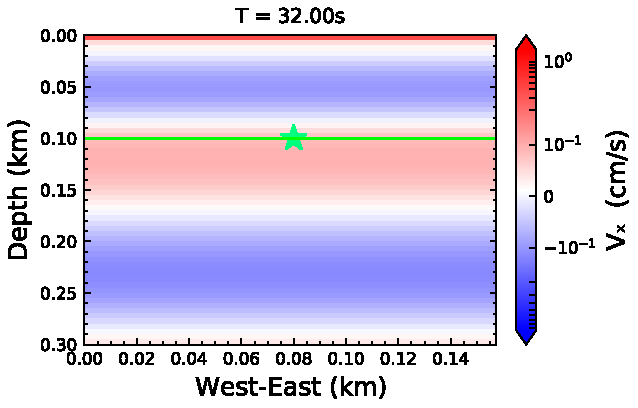
\includegraphics[width=0.4\textwidth]{figures/figure_etf_S3b.pdf}\label{fig:etf-S3f}} \\[\baselineskip]%

  \caption{Snapshots of ${V_X}$ at TKCH05 along the A-A' cross section in \Cref{fig:etf-8}c, bandpass filtered between 4.5 and 5 Hz. (a), (c) and (e) display snapshots of the 3D model, where the gray contour lines represent interfaces between bulks with difference Vs; the green star denotes the downhole site and the green line marks its depth. (b), (d) and (f) are for the 1D model.}
  \label{fig:etf-S3}
\end{figure}

\clearpage
\floatsetup[figure]{style=plain,subcapbesideposition=top}
\begin{figure}[!ht]
  \sidesubfloat[]{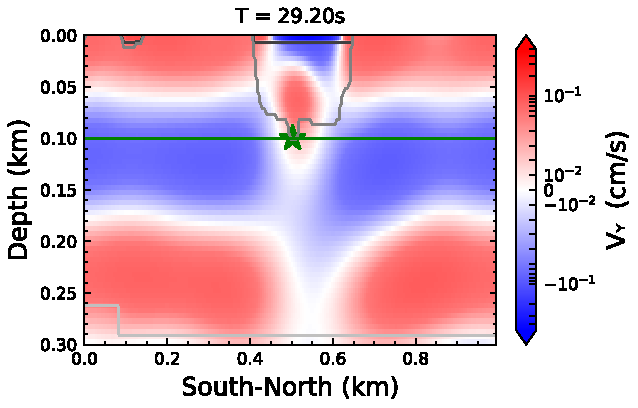
\includegraphics[width=0.4\textwidth]{figures/figure_etf_S4a.pdf}\label{fig:etf-S4a}} \hfil
  \sidesubfloat[]{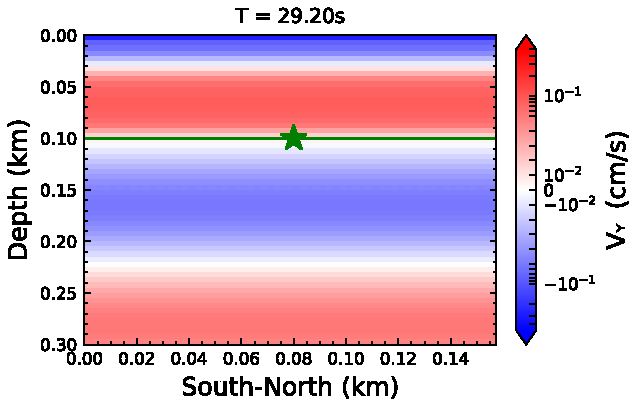
\includegraphics[width=0.4\textwidth]{figures/figure_etf_S4b.pdf}\label{fig:etf-S4b}} \\[\baselineskip]%
  \sidesubfloat[]{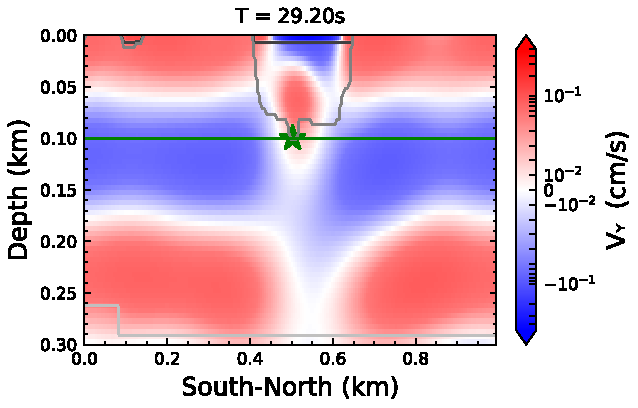
\includegraphics[width=0.4\textwidth]{figures/figure_etf_S4a.pdf}\label{fig:etf-S4c}} \hfil
  \sidesubfloat[]{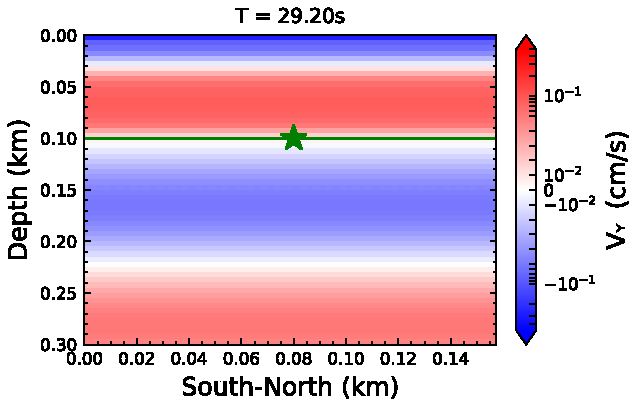
\includegraphics[width=0.4\textwidth]{figures/figure_etf_S4b.pdf}\label{fig:etf-S4d}} \\[\baselineskip]%
  \sidesubfloat[]{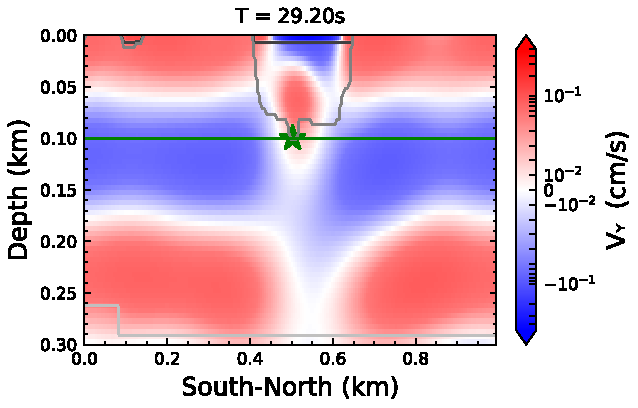
\includegraphics[width=0.4\textwidth]{figures/figure_etf_S4a.pdf}\label{fig:etf-S4e}} \hfil
  \sidesubfloat[]{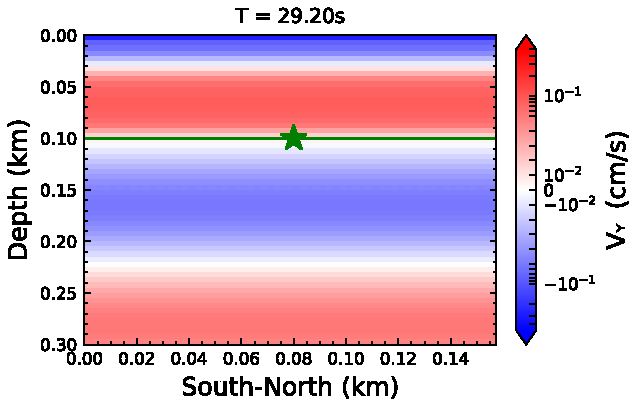
\includegraphics[width=0.4\textwidth]{figures/figure_etf_S4b.pdf}\label{fig:etf-S4f}} \\[\baselineskip]%

  \caption{Same as \Cref{fig:etf-S3}, except along the B-B’ cross section in \Cref{fig:etf-8}c.}
  \label{fig:etf-S4}
\end{figure}

% \clearpage
% \section*{Appendix}\label{app:2-1}
% \addcontentsline{toc}{section}{\protect\numberline{}Appendix}

% The form of the Von Karman autocorrelation function \citep{frankel_finite_1986} is

% \begin{equation}\label{eq:2-A1}
%   \Phi_{v, a}(r)=\sigma^{2} \frac{2^{1-v}}{\Gamma(v)}\left(\frac{r}{a}\right)^{v} K_{v}\left(\frac{r}{a}\right)
% \end{equation}

% \noindent in which $\nu$ is the Hurst component, $a$ is the correlation length, $K_{\nu}$ is the modified Bessel function of order $\nu$, $\Gamma(\nu)$ is the gamma function, and $\sigma^2$ is the variance with Fourier transform:

% \begin{equation}\label{eq:2-A2}
%   P(k)=\frac{\sigma^{2}(2 \sqrt{\pi} a)^{E} \Gamma(v+E / 2)^{v+E / 2}}{\Gamma(v)\left(1+k^{2} a^{2}\right)}
% \end{equation}

% \noindent in which $E$ is the Euclidean dimension.


% %% Bibilography
% \newpage
% \linespread{1.0}
% \setlength\bibitemsep{2\itemsep}
% \AtNextBibliography{\normalsize}
% \addcontentsline{toc}{section}{\protect\numberline{}References}
% \printbibliography[section=\therefsection,title=References, heading=subbibliography]

\renewcommand{\thetable}{\arabic{table}}
\renewcommand{\thefigure}{\arabic{figure}}

\numberwithin{figure}{chapter}
\numberwithin{table}{chapter}

%\endrefsection